\documentclass[twocolumn,preprintnumbers]{aastex6} 
\bibliographystyle{unsrt}

\usepackage{afterpage}
\usepackage{capt-of}
\usepackage{diagbox}

\usepackage[figuresright]{rotating}
\usepackage{amsmath}
\usepackage{amssymb,amsmath,latexsym,graphics, graphicx,epsfig,multirow,comment,hyperref,appendix,feyn,slashed,xcolor,afterpage, makecell} 
\usepackage{booktabs}
\usepackage{tabularx}
\usepackage{wasysym}



\newcommand{\grp}[1]{\mathrm{#1}}

\newcommand{\grO}{\grp{O}}
\newcommand{\grU}{\grp{U}}
\newcommand{\grSU}{\grp{SU}}
\newcommand{\grSO}{\grp{SO}}
\newcommand{\grUSp}{\grp{USp}}
\newcommand{\grE}{\grp{E}}
\newcommand{\grSL}{\grp{SL}}
\newcommand{\HH}{\mathbb{H}}

\newcommand{\FeH}{\text{[Fe/H]} }
\newcommand{\alphaFe}{\text{[$\alpha$/Fe]} }

\newcommand{\norm}[1]{\left\lVert #1 \right\rVert}
\newcommand{\abs}[1]{\left\lvert #1 \right\rvert}
\newcommand{\overbar}[1]{\mkern 2mu\overline{\mkern-2mu#1\mkern-2mu}\mkern 2mu}

\newcommand {\be} {\begin {equation}}
\newcommand {\ee} {\end {equation}} 
\newcommand {\nn} {\nonumber}
\newcommand {\bes} {\begin {equation*}}
\newcommand {\ees} {\end {equation*}}
\newcommand {\trit} {^3\text{H}}

\newcolumntype{L}[1]{>{\raggedright\let\newline\\\arraybackslash\hspace{0pt}}m{#1}}
\newcolumntype{C}[1]{>{\centering\let\newline\\\arraybackslash\hspace{0pt}}m{#1}}
\newcolumntype{R}[1]{>{\raggedleft\let\newline\\\arraybackslash\hspace{0pt}}m{#1}}

\newcommand{\es}[2] {\begin{equation} \label{#1} \begin{split} #2 \end{split} \end{equation}}

\usepackage{csvsimple}
\newcommand{\CP}{\mathbb{CP}}
\newcommand{\Z}{\mathbb{Z}}
\newcommand{\N}{\mathbb{N}}
\newcommand{\R}{\mathbb{R}}
\newcommand{\C}{\mathbb{C}}

\newcommand{\Gr}{\mathrm{Gr}}

% define "struts", as suggested by Claudio Beccari in
%    a piece in TeX and TUG News, Vol. 2, 1993.
\newcommand\Tstrut{\rule{0pt}{2.6ex}}         % = `top' strut
\newcommand\Bstrut{\rule[-0.9ex]{0pt}{0pt}}   % = `bottom' strut


\makeatletter
\newcommand\footnoteref[1]{\protected@xdef\@thefnmark{\ref{#1}}\@footnotemark}
\makeatother


\def\CA{{\cal A}}
\def\CB{{\cal B}}
\def\CC{{\cal C}}
\def\CD{{\cal D}}
\def\CE{{\cal E}}
\def\CG{{\cal G}}
\def\CH{{\cal H}}
\def\CI{{\cal I}}
\def\CK{{\cal K}}
\def\CL{{\cal L}}
\def\CR{{\cal R}}
\def\CM{{\cal M}}
\def\CN{{\cal N}}
\def\CO{{\cal O}}
\def\CP{{\cal P}}
\def\CQ{{\cal Q}}
\def\CW{{\cal W}}

\DeclareRobustCommand{\Sec}[1]{Sec.~\ref{#1}}
\DeclareRobustCommand{\Secs}[2]{Secs.~\ref{#1} and \ref{#2}}
\DeclareRobustCommand{\Secss}[3]{Secs.~\ref{#1}, \ref{#2}, and \ref{#3}}
\DeclareRobustCommand{\App}[1]{App.~\ref{#1}}
\DeclareRobustCommand{\Tab}[1]{Table~\ref{#1}}
\DeclareRobustCommand{\Tabs}[2]{Tables~\ref{#1} and \ref{#2}}
\DeclareRobustCommand{\Fig}[1]{Fig.~\ref{#1}}
\DeclareRobustCommand{\Figs}[2]{Figs.~\ref{#1} and \ref{#2}}
\DeclareRobustCommand{\Figss}[3]{Figs.~\ref{#1}, \ref{#2}, and \ref{#3}}
\DeclareRobustCommand{\Eq}[1]{Eq.~(\ref{#1})}
\DeclareRobustCommand{\Eqs}[2]{Eqs.~(\ref{#1}) and (\ref{#2})}
\DeclareRobustCommand{\Ref}[1]{Ref.~\cite{#1}}
\DeclareRobustCommand{\Refs}[1]{Refs.~\cite{#1}}

\newcommand{\upstate}{\left|\uparrow \right\rangle}
\newcommand{\downstate}{\left|\downarrow \right\rangle}

\def\arccosh{\mop{arccosh}}

\newcommand{\beq}{\begin{equation}}
\newcommand{\eeq}{\end{equation}}

\newcommand {\kms} {\,\,\text{km}/\text{s}}
\newcommand{\V}[1]{{ \bf #1}}
\newcommand{\obs}{\text{obs}}
\newcommand{\Min}{\text{min}}
\newcommand{\erf}{\text{erf}}
\newcommand{\esc}{\text{esc}}
\newcommand{\kevee}{\text{keV}_{\text{ee}}}
\newcommand{\cpdkg}{\, \, \text{cpd} \,\text{kg}^{-1}}
\newcommand{\flow}{\text{flow}}
\newcommand{\kevnr}{\, \, \text{keV}_\text{nr}}
\newcommand{\CNB}{\text{C}\nu\text{B}}
\newcommand{\zacc}{z_\mathrm{acc}}
\def\ML#1{\textcolor{red}{[ML: #1]}}
\def\lmn#1{\textcolor{blue}{[LN: #1]}}

\newcommand{\mi}{\texttt{m12i}}
\newcommand{\mf}{\texttt{m12f}}

\begin{document}

\title{
Firing up the Local Dark Matter Distribution from the Stars
}

\author{Lina Necib}
\affil{Walter Burke Institute for Theoretical Physics,
California Institute of Technology, Pasadena, CA 91125, USA}


\author{Mariangela Lisanti}
\affil{Department of Physics, Princeton University, Princeton, NJ 08544}

\author{Shea Garrison-Kimmel}
\affil{TAPIR, Mailcode 350-17, California Institute of Technology, Pasadena, CA 91125, USA}
\author{Andrew Wetzel}
\affil{Department of Physics, University of California, Davis, CA 95616, USA}
\author{Robyn Sanderson}
%\affil{TAPIR, Mailcode 350-17, California Institute of Technology, Pasadena, CA 91125, USA}
\author{Phillip Hopkins}
\affil{TAPIR, Mailcode 350-17, California Institute of Technology, Pasadena, CA 91125, USA}

\begin{abstract}
In this paper, we use two hydrodynamic zoom-in simulations of the Milky Way from the FIRE suite with different merger histories to establish a strong correlation between the velocity distribution of the luminous accreted component of dark matter and that of the stars, accreted in the same events. We are therefore able to \emph{empirically} extract the velocity distribution of the virialized dark matter component, as well as that of the largest contributing mergers from the stars. As such mergers contribute different amounts of stars and dark matter,  we used the mass-metallicity relation as well as the mass to light ratios in the simulations to find the relative contribution of each merger to the virialized component. We finally extend this strategy to the Milky Way, and apply our findings to the recently found velocity distribution of a large local debris flow referred to as the Gaia Sausage. Smoothly accreted dark matter as well as dark matter from dark subhalos cannot be inferred using this method as such events do not contain stars.
\end{abstract}
\maketitle
\pagebreak

\section{Introduction} 
\label{sec:intro}

In the $\Lambda$CDM paradigm, dark matter (DM) halos are built up hierarchically from smaller, satellite galaxies that merge with the host halo~\citep{1978MNRAS.183..341W,Diemand:2008in,Springel:2008cc,2011ApJ...740..102K}, the oldest of which may also contribute stars that populate the stellar halo~\citep{Johnston:1995vd, Johnston:1996sb, Helmi:1999ks, Bullock:2000qf, Bullock:2005pi, Purcell:2007tr, DeLucia:2008gk}. Due to their common origin, the stellar halo can hold clues to understanding the DM distribution in the Milky Way.  In this work, we use the \textsc{Feedback in Realistic Environments (Fire)} hydrodynamic simulations~\citep{2014MNRAS.445..581H, 2017arXiv170206148H} to study the correlation between the DM and stellar halos and its dependence on the galactic merger history.

The chemical abundance and phase-space distribution of stars can be used to infer properties of its satellite progenitor~\citep{Helmi:2002iu, 2005ApJ...635..931B, Robertson:2005gv, Font:2005qs, DeLucia:2008gk, 2016ApJ...821....5D}.  Based on the large radial anisotropy and metallicity of inner-Galaxy stars (within $\sim20$~kpc) it was recently shown that they are dominated by the merger of a large satellite galaxy with stellar mass $M_* \sim 10^{7-8}$~M$_\odot$ at redshift $\sim 1$--3~\citep{2018arXiv180203414B}.  This merger can explain the observed density break at Galactocentric radii of $\sim 20$~kpc as well as the population of globular clusters on highly radial orbits.  Referred to as the \emph{Gaia} Sausage, the contribution of this substructure population comprises approximately 60\% of the local distribution of accreted stars, with the remaining fraction appearing to be nearly isotropic and very metal poor~\citep{necib2018}.  There is also evidence for smaller stellar streams in the vicinity of the Solar neighborhood~\citep{Myeong:2017skt}.

The goal of this work is to understand how well the accreted stars act as tracers for the underlying kinematic DM distribution that is also sourced from the same merger events.  This correspondence is not guaranteed by default for a variety of reasons.  First, while any given satellite galaxy contributes DM and stellar debris, the stars are more tightly bound towards the center.  Therefore, only DM is stripped off initially as the outer regions of the satellite are eaten away.  Additionally, the mass to luminosity relation varies between galaxies, so the relative number of stars to DM that each contributes may vary.  

In previous work, a subset of the authors studied the stellar-DM correspondence in \textsc{Eris} hydrodynamic simulation of a Milky Way-like galaxy.  The focus in this case was on reconstructing the virialized DM distribution, and they found excellent correspondence in the velocity distributions as more metal-poor stars were selected, with convergence reached for stars with $\FeH < -3$ \citep{Herzog-Arbeitman:2017fte}.  This result was later used to infer the local virialized DM velocity distribution in data using RAVE-TGAS~\citep{Herzog-Arbeitman:2017zbm}. However, the question remains as to how generic this result is and whether it depends on the detailed formation history of the halo or the DM properties themselves. 

Additionally, one would also be interested in how well the DM and stars from younger mergers trace each other.  These mergers can leave distinctive features in the position and velocity distribution.  For example, streams result from the tidal debris torn off a satellite as it completes a small number of orbits.  In this case, the stream typically traces out parts of the progenitor's orbit \citep{2012JCAP...08..027P}.  Debris flow is an example of kinematic substructure that results after a satellite completes many more  orbital wraps \citep{Lisanti:2011as,Kuhlen:2012fz}.  In this case, any structure in position-space is washed out, while velocity-space features remain.  

Simulations of the Sagittarius stream suggest that the correlation between the stars and DM may not be exact, with spatial offsets between the two and the DM being more dispersive \citep{2012JCAP...08..027P}.  Debris flow, on the other hand, seems to be quite similar between stars and DM, likely because the merger event is older and the debris is more well-mixed.  However, these conclusions are based on studies of the Via Lactea DM-only simulation where star `particles' were painted onto the most bound DM particles in the satellite galaxies.

Our approach in this work is to identify the stars and DM that originate from a given satellite galaxy in the simulation and to trace them as a function of time to see where they eventually end up relative to each other.  Following this procedure over the largest mergers in the galaxy, we can carefully study how the DM  and stellar halos are built up.  This is the first study of its kind performed using a hydrodynamic simulation of a Milky-Way--like galaxy.  


\begin{comment}
High resolution $N$-body simulations that track the formation of Milky-Way--like halos have demonstrated the breadth of possibilities for the local DM distribution.  DM-only simulations have shown that, while halos are built from the inside out~\citep{Zhao:2002rm}, the history of our own special neighborhood within the Galaxy can vary considerably depending on the number of recent mergers that contribute tidal debris to the region~\citep{Diemand:2007qr, 2011MNRAS.413.1373W}.  This manifests in a wide range of possibilties for the local DM phase-space distribution
~\citep{Vogelsberger:2007ny, Vogelsberger:2008qb, Kuhlen:2009vh, Kuhlen:2012fz}.  More recently, hydrodynamic $N$-body simulations that trace the DM, as well as gas and stars, have started to reach comparable resolutions~\citep{Ling:2009eh, 
Guedes:2011ux, 2013ApJ...773...43B,
2014MNRAS.445..581H,
Schaye:2014tpa, 2015MNRAS.450.1937C, Schaller:2015vsa,
Wang:2015jpa, Sawala:2015cdf,
2017arXiv170206148H,Monachesi:2018xya}.  The effect of baryons tends to virialize the DM distributions faster~\citep{Kelso:2016qqj, Pillepich:2014784, Butsky:2015pya, },
although considerable variation in the local phase-space distributions is still observed between these simulations.
%FIRE accretion history~\cite{2017arXiv171203966G}
\end{comment}

We study the DM and stellar halos in two Milky-Way--like halos in the suite of \textsc{Fire} simulations.  
This builds off of previous studies by using two new halos with rather different merger histories to each other.  Additionally, we use the full history of the simulation output to study how the relation between DM and stars depends on accretion time. \ML{some words on FIRE?}

We find that stars from the oldest mergers trace the virialized component of the DM distribution. Stars and DM from the same merging events are also closely related in the case of debris flows, though offsets lead to different in the velocity distributions of streams, but not that of the speed distribution. 
Since each merging event contributes a different amount of DM and stars, we used an empirical mass to light ratio along with a mass-metallicity relation in the simulations to obtain a relationship between the average metallicity of a merging subhalo and the ratio of the total subhalo mass to its stellar mass. Using such relation, we can rescale the velocity distribution of a particular merger to that of the virialized component and obtain the DM velocity distribution from the largest mergers, normalized by their proper contribution. We cannot however extrapolate the contributions from the dark subhalos and smoothly accreted DM, which we leave to future study.


This paper is organized as follows. Sec.~\ref{sec:fire} introduces the \textsc{Fire} simulations and provides more details about the two halos studied in detail here.  Sec.~\ref{sec:origins} describes the breakdown of the DM and stars in the local volume in terms of their accretion time and progenitor mass. In \Sec{sec:correlation}, we establish the correlation between the stars and DM for both the virialized components, and the individual mergers, and in \Sec{sec:totaldarkmatter} we discuss the building blocks of the DM distribution, including smoothly accreted DM and dark subhalos, which cannot be tracked using stars. Finally, we apply this new strategy to the Milky Way in \Sec{sec:milky_way}.




\section{FIRE Simulations}
\label{sec:fire}

We analyze two cosmological, hydrodynamic zoom-in simulations \citep{KatzWhite1993,Onorbe2014} from the \textsc{Latte} sample \citep{Wetzel2016}, part of the \textsc{Feedback in Realistic Environments} (\textsc{Fire})\footnote{\url{http://fire.northwestern.edu}} project.  The simulations were run with the \textsc{Fire-2} version of the code~\cite{2017arXiv170206148H} and use the \textsc{Gizmo} \citep{Hopkins:2014qka} code,\footnote{\url{http://www.tapir.caltech.edu/~phopkins/Site/GIZMO.html}} with hydrodynamics solved using the mesh-free Lagrangian Godunov ``MFM'' method. Both hydrodynamic and gravitational (force-softening) spatial resolution are set in a fully-adaptive Lagrangian manner and the mass resolution is fixed. The simulations include cooling and heating from a meta-galactic background and local stellar sources from $T\sim10-10^{10}$~K.  Star formation occurs in locally self-gravitating, dense,  and self-shielding molecular, Jeans-unstable gas.  Stellar feedback occurs through OB \&\ AGB mass-loss, SNe Ia \&\ II, and multi-wavelength photo-heating and radiation pressure, with inputs taken directly from stellar evolution models\ML{which ones?}. The physics, source code, and numerical parameters are nearly identical to those in \citet{2017arXiv170206148H}, but here we analyze simulations that additionally include a sub-grid prescription for turbulent metal diffusion \citep{2017arXiv170206148H,Escala2017}.  \ML{Don't we need some more detailed info on how the metallicities are determined?}

This work focuses specifically on \textsc{FIRE} galaxies \texttt{m12i} and \texttt{m12f}, which are Milky-Way--like halos.   Both assume $\Lambda$CDM cosmology with $h\approx 0.70$, $\Omega_M \approx 0.27$, and $\Omega_b \approx 0.045$~\citep{Ade:2013zuv}.  Both simulations consist of \ML{fill in} DM, gas, and star particles.  The baryonic particles have mass $\sim 7\times10^{3}$~M$_\odot$ and gravitational softening length of 4~pc; the DM particle mass if $3.5 \times10^4$~M$_\odot$ and have a 20~pc softenting length.  The primary host halo in \texttt{m12i} has a virial mass of $1.2\times10^{12}$~M$_\odot$, a virial radius of 275~kpc, and stellar mass of $6.5\times10^{10}$~M$_\odot$.  
The corresponding properties of \texttt{m12f} are $1.6\times10^{12}$~M$_\odot$, 306~kpc, and $8.0\times10^{10}$~M$_\odot$, respectively. 
\ML{Make some statements comparing the general features of m12i and m12f to the Milky Way}

DM subhalos are identified using the \textsc{Rockstar} halo finder~\citep{Behroozi:2011ju}.\footnote{\url{https://bitbucket.org/pbehroozi/rockstar-galaxies}}\ldots \ML{more details}
%
The actual procedure of identifying a DM or star particle with a given subhalo is different.  For stars, we run rockstar\footnote{\url{https://bitbucket.org/gfcstanford/rockstar/src/master/}} \citep{2013ApJ...762..109B} on the DM particles only, find the DM subhalos, then associate the stars within each subhalo, matching them in phase-space \lmn{Ask Andrew about details here}. For the DM particles, we look at the particles within the virial radius of the each subhalo found in rockstar.  




%
%\begin{figure*}[tb] %  figure placement: here, top, bottom, or page
%   \centering
%		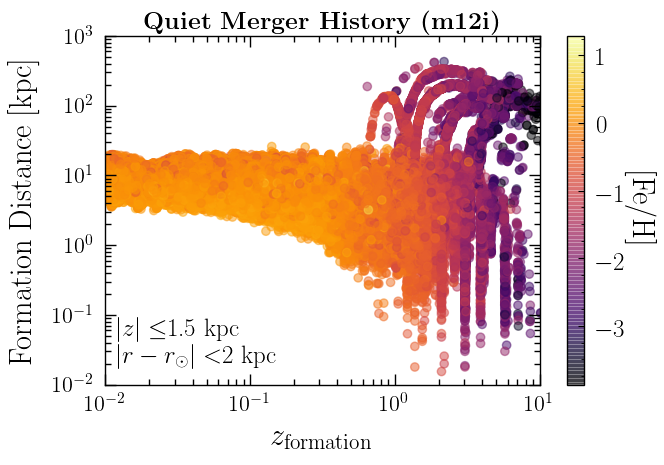
\includegraphics[width=0.40\textwidth]{plots/form_distance_age_m12i.png} 
%		\qquad
%		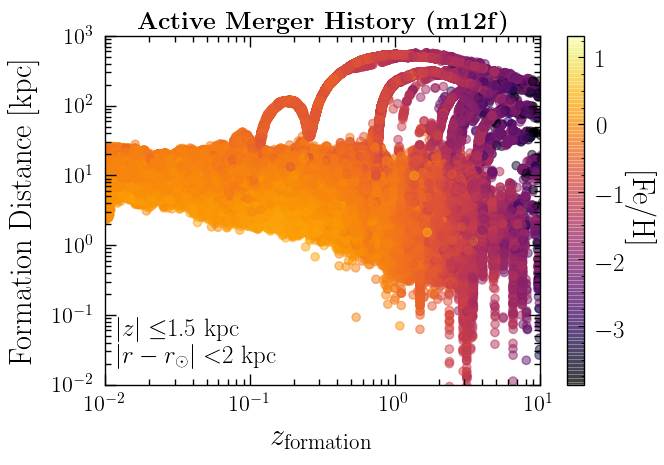
\includegraphics[width=0.40\textwidth]{plots/form_distance_age_m12f.png} 
%   \caption{Formation distance and redshift for all stars within the local volume of host halo \texttt{m12i} (left) and \texttt{m12f} (right).  The color denotes the iron abundance, $\FeH$, of each star.  The local volume is defined as $|z|\leq 1.5$~kpc and $|r-r_\odot|\leq 2$~kpc, where $z$ is the vertical distance off the galactic plane, $r$ is the galactocentric radius, and $r_\odot = 8$~kpc is the solar position. \ML{Update to pdf}}
%   \label{fig:formation}
%\end{figure*}



\section{Accretion History in the Solar Neighborhood}
\label{sec:origins}

\begin{table*}[t]
\centering
\footnotesize
\renewcommand{\arraystretch}{1.5}
\begin{tabular}{C{4 cm} | C{1.3cm} C{1.3cm} C{1.3cm}C{1.3cm} | C{1.3cm} C{1.3cm} C{1.3cm}C{1.3cm}}
\Xhline{3\arrayrulewidth}
&\multicolumn{4}{c|}{\textbf{\texttt{m12i} Host Halo}} &  \multicolumn{4}{c}{\textbf{\texttt{m12f} Host Halo}} \\
 &   I & II & III & IV & I & II & III & IV    \\ 
 \hline
 $M_\mathrm{Peak}$~[M$_\odot$] & $2.4\times10^9$ & $5.2\times10^{10}$ & $1.7 \times 10^{10}$ & $3.4\times10^{10}$ & $6.0 \times 10^8$ & $3.8\times10^8$ & $7.4\times10^{10}$ & $2.4\times10^{10}$ \\
 $z_\mathrm{acc}$ & 2.0 & 1.5 & 3.0 & 2.5 & 0.1 & 0.7 & 0.8 & 0.2 \\
 $\langle \FeH \rangle$ & $-1.58$ & $-1.55$ & $-1.83$ & $-1.97$ & $-0.80$ & $-0.95$ & $-1.17$ & $-1.01$ \\
 $M_\mathrm{Peak}/M_\mathrm{sub, *}$ & 82 & 89 & 115 & 122 & 8.8 & 43 & 46 & 47 \\
Stellar Mass Fraction (ROI) & 32\% & 30\% & 15\% & 7\% & 40\% & 23\% & 13 \% & 7\% \\
DM Mass Fraction (ROI) & 3.2\% & 4.9\% & 4.2\% & 10\% & 7.6\% & 6.3\% & 9.0\% & 1.0\% \\
DM to Star Mass Ratio (ROI) & 1.38 & 2.25 & 3.90 & 21.0 & 0.90 & 1.34 & 3.52 & 0.74 \\
% I  &  $2.4\times 10^9$ & 2.0 & -1.58 & 0.32 & 1.38 & 82 & $6.0 \times 10^8$ & 0.1 & -0.80 & 0.40 & 0.90 & 8.8\\ \hline
 %II  & $5.2 \times 10^{10}$ & 1.5 & -1.55 & 0.30 & 2.25 & 89 & $3.8  \times 10^{8}$ & 0.7 & -0.95 &0.23 & 1.34 & 43 \\ \hline
 %III  & $1.7 \times 10^{10}$ & 3.0 & -1.83 & 0.15  & 3.90 & 115 & $7.4 \times10^{10}$ & 0.8 & -1.17 & 0.13 & 3.52 & 46\\ \hline
% IV &  $3.4 \times 10^{10}$ & 2.5 & -1.97 & 0.07 & 21.0 & 122 & $2.4 \times 10^{10}$ & 0.2 & -1.01 & 0.07 & 0.74 & 47 \\
    \Xhline{3\arrayrulewidth}
  \end{tabular}
  \caption{Properties of the top four satellite galaxies (labeled as I-IV) in \mi~and~\mf, ranked by the fraction of stellar mass each contributes to the local volume.  For each galaxy, we list the peak mass of its dark matter halo ($M_\mathrm{sub}$), accretion redshift ($z_{\rm{acc}}$), average stellar metallicity ($\langle \FeH \rangle$), and halo-to-stellar mass ratio ($M_\mathrm{sub}/ M_{\mathrm{sub}, *}$).  We also provide the stellar mass fraction and the fraction of dark matter to star particles contributed by the satellite galaxy within the local volume (ROI).  The dominant mergers in \mf~are all more recent than those of \mi.  }
  \label{tab:progenitors}
  \end{table*}

In this work, we study the correlation of the DM and stellar phase-space distributions for Milky-Way--like halos.  As our focus is on the DM in the solar neighborhood, we restrict our study to the volume within distances $|z| \leq 1.5$~kpc off the plane and galactocentric radii $r_{\odot} \pm 2$~kpc, where $r_\odot = 8$~kpc.\footnote{Alternatively, one can rescale the distance from the sun to the center of the galaxy by the virial radius of each simulated host halo, but we choose to adopt the same convention as \cite{2018arXiv180610564S}.} In this volume, there are a total of $\sim 1.70\times 10^5$($2.19\times10^5$) DM and $\sim 9.78\times10^5$($1.48\times10^6$) star particles in \mi(\mf).  % \{DM, star\} $=\{170462, 978754 \}$ and $\{219406 , 1476680 \}$ particles in \texttt{m12i} and \texttt{m12f}, respectively.

\begin{figure*}[tb] %  figure placement: here, top, bottom, or page
   \centering
		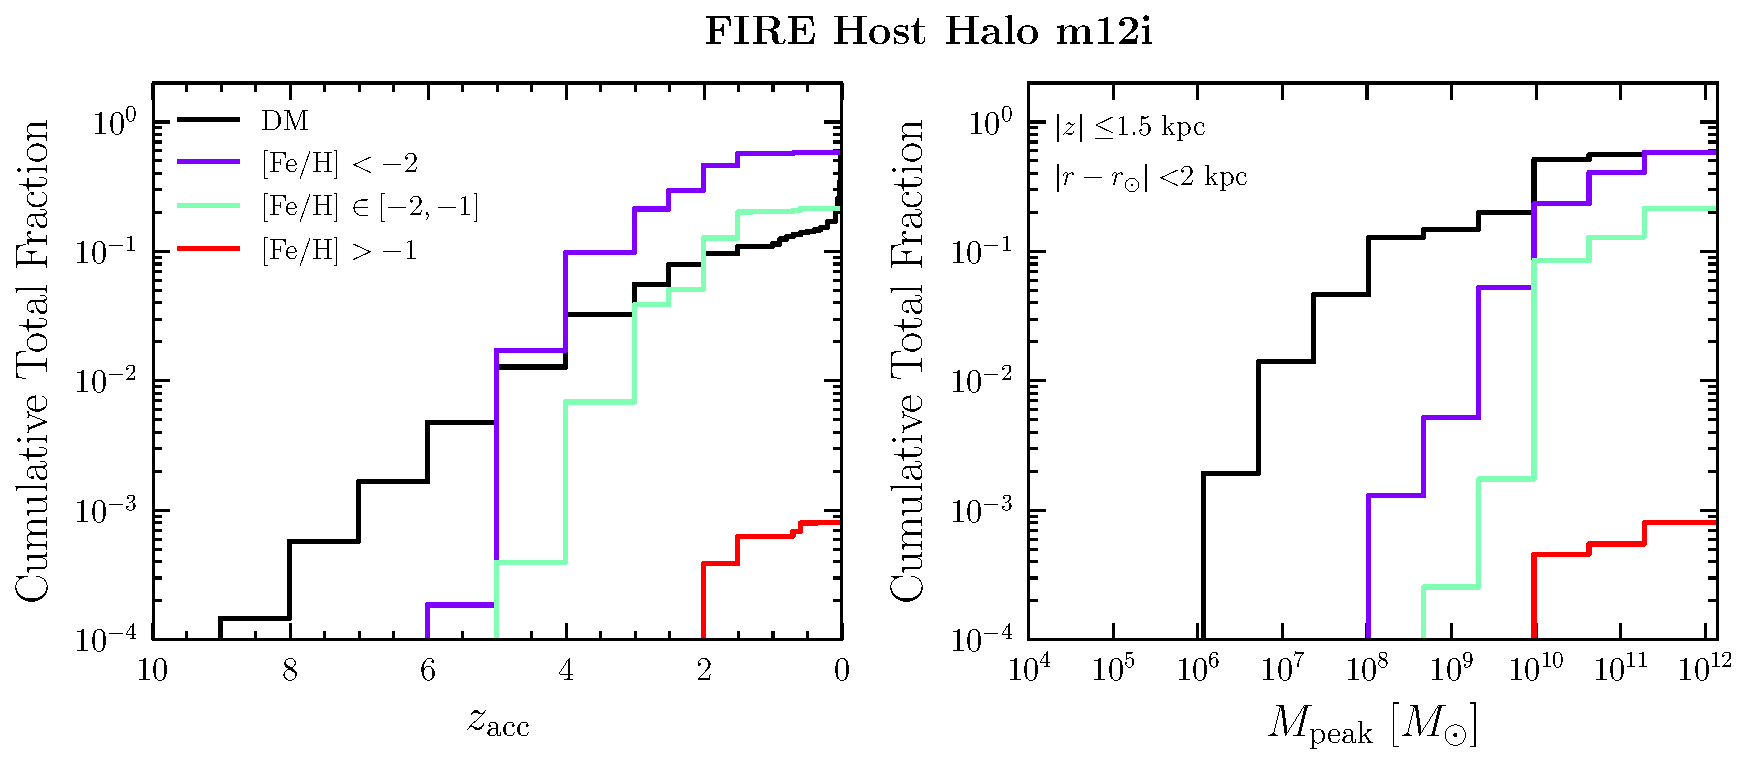
\includegraphics[width=0.85\textwidth]{plots/particle_origins_cumulativem12i.pdf} 
		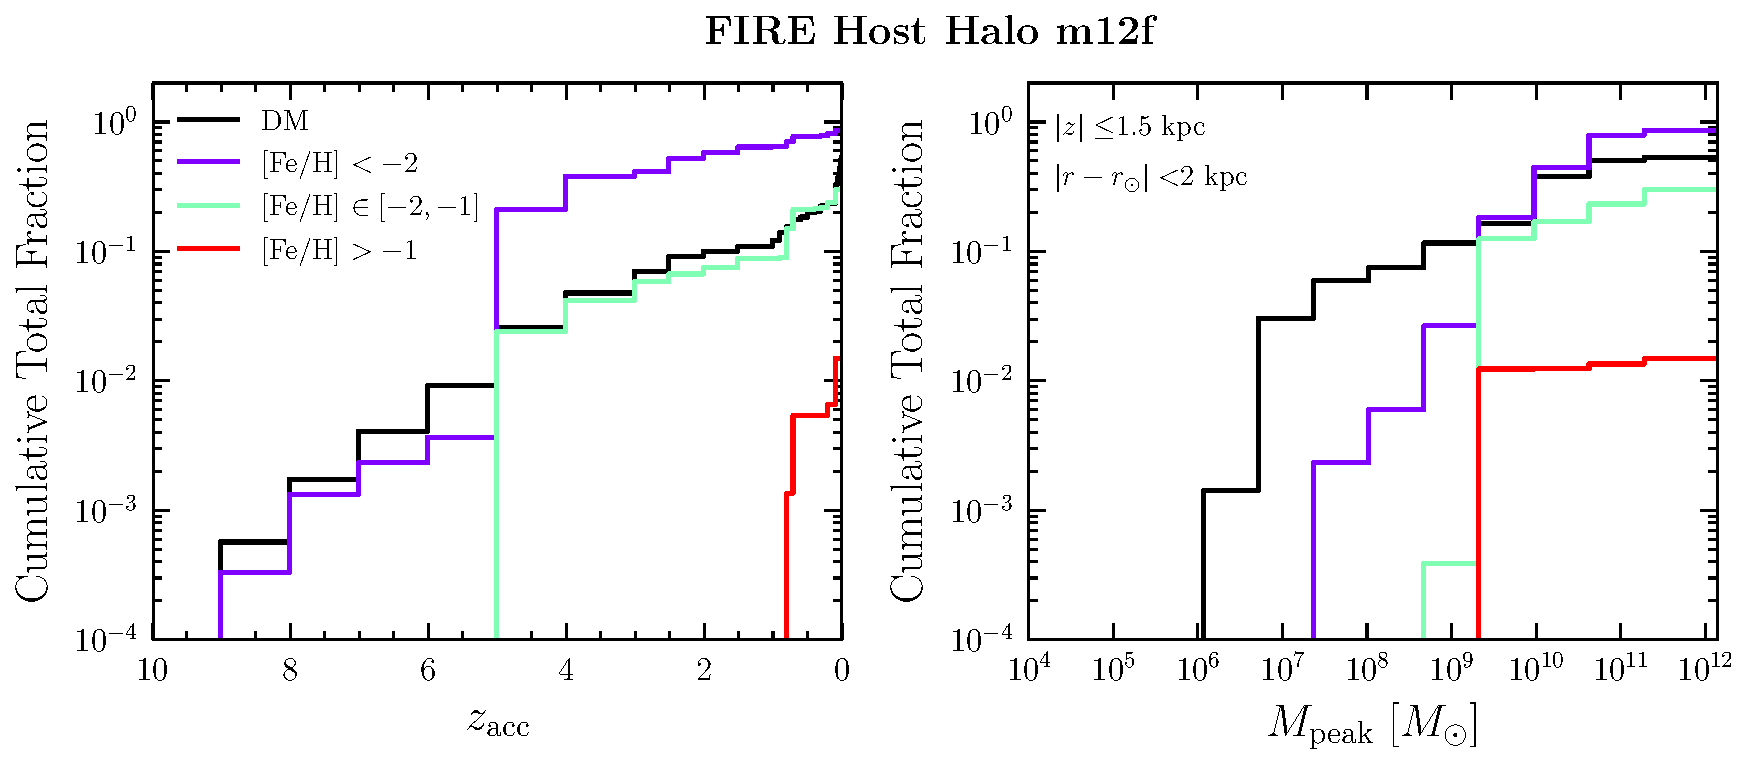
\includegraphics[width=0.85\textwidth]{plots/particle_origins_cumulativem12f.pdf} 
   \caption{The origin of the DM and stars in the local volume of host \texttt{m12i} (top) and \texttt{m12f} (bottom) that have been accreted from merging satellites.  The cumulative fraction of dark matter (black lines) and stars is shown as a function of accretion redshift (left) and progenitor mass (right).  The stars are broken down into different metallicity ranges: $\FeH > -1$, $\FeH \in [-2,-1]$, and $\FeH < -2$, indicated by the red, acqua, and purple lines, respectively.  The cumulative fraction is defined with respect to the total number of particles of each kind found in the local volume at $z=0$.  The deficit below unity at $\zacc = 0$ (or $M_\mathrm{Subhalo} = 10^{12}$~M$_\odot$) corresponds to the diffuse fraction for the DM and the \emph{in-situ} fraction for the individual stellar components.  Note that the DM particle mass in the simulation is $\sim 7~10^4$~M$_\odot$, so that subhalo masses below $\sim \rm{few} ~10^5 M_{\odot}$ are not resolved.}
   \label{fig:origins}
\end{figure*}
 
Given the simulation output, it is possible to track the location of a DM/star particle over all time stamps.\footnote{\ML{provide brief description of total number of time stamps and average spacing.}} To start, we identify all the DM and star particles in the local volume of the host at the present day.  We then follow the location of each particle at incrementally larger redshifts, verifying whether it is bound to a subhalo at a given time stamp.  If it is, we mark the subhalo as its parent and the time stamp as the particle's accretion redshift, $\zacc$.  Note that the value of $\zacc$ is only approximate, as the actual accretion time may have occurred between time stamps, but it serves as an adequate approximation for our purposes. 

In this manner, we identify the subhalo progenitor of each DM/star particle observed in the local volume of the host galaxy.  We also  collect information on the progenitor halo, such as its total DM and stellar mass. Due to tidal stripping, the total mass of a subhalo at $\zacc$ is typically smaller than its true infall mass.  A more accurate estimate of the infall mass can be obtained by tracking the particle to earlier time stamps and finding the progenitor's peak mass.

We note that some fraction of the DM in the local volume originated from smooth accretion, meaning that it became bound to the host at $\zacc$, but was not bound to any other subhalo prior to that time.  We find that approximately 30\% of the DM in the local volume of \texttt{m12i} falls in this category, compared to 50\% for \texttt{m12f}.  In both cases, the diffuse component was accreted at $\zacc <1.5$.  A large caveat here is that some particles might have not been correctly identified as belonging to a particular subhalo, and this might affect our results, although since we only required the DM particles to be within the virial radius of the subhalos, without any cut on their velocity, we expect to be more skewed towards having smoothly accreted particles mistakenly associated with subhalos. Another issue is that due to the resolution of the simulation, some of the DM that we attribute to smooth accretion may acction originate from small subhalos below the simulation's resolution.

Table~\ref{tab:progenitors} lists the top four satellite galaxies  that contribute the greatest fraction of stellar debris in the local volume of \texttt{m12i}.  We see that 32\% of the stellar mass fraction is due to debris from a $\sim 2 \times 10^9$~M$_\odot$ subhalo at $z_\text{acc} = 2$.  The next most significant merger contributes 30\% of the stellar mass; it occurred later at $\zacc = 1.5$ and was due to a more massive progenitor with mass $\sim 5\times 10^{10}$~M$_\odot$.  In contrast, the majority of the local stellar halo in \mf~was accreted at lower redshifts.  
For example, $\sim$40\% of the stellar mass fraction in the local volume of \texttt{m12f} arises from a $\sim 6\times 10^8$~M$_\odot$ subhalo at redshift $0.1$, while the next 23\% is due to a $\sim4\times10^8$~M$_\odot$ halo at $\zacc = 0.7$.  

Because the dominant mergers in \mf~are younger relative to those of \mi, they are typically more luminous with smaller $M_\mathrm{sub}/M_\mathrm{sub,*}$.  Also, the average metallicity of their stars are more metal-rich than those of \mi.  For both host galaxies, mergers I-IV contribute nearly all of the local stellar mass, but a much smaller fraction of the local DM.  For example, the top four mergers in either \mi or \mf~contribute $\sim85\%$ of the accreted stars, but only contribute $\sim20\%$ of the accreted DM. This is consistent with the fact that stellar halos form through the largest mergers, while DM halos form more progressively through a larger range of subhalos \citep{}.
%The next largest contribution (23\% of the total) is due to a subhalo of mass $3.8\times 10^8$ at redshift 0.7.  

The top left panel of Fig.~\ref{fig:origins} illustrates how the cumulative fraction of DM and stars in \mi~(relative to all the particles of the same type in the local volume at $z=0$) grows with time.  By redshift 0, the total fraction of accreted stars in each metallicity bin [Fe/H]$>-1$,  [Fe/H]$\in [-2, -1]$, and [Fe/H]$<-2$ is approximately 0.08\%, 22\%, and 60\%, respectively.  Clearly, very few metal-rich stars originate from mergers and the accreted stellar fraction increases considerably towards the more metal-poor end of the spectrum.   Additionally, we observe that the majority of accreted stars---regardless of their metallicity---are in place by redshift $\sim2$. 

The bottom panel of Fig.~\ref{fig:origins} shows the corresponding cumulative histograms for host \texttt{m12f}.  The relative contributions from stars of different metallicities is distinct from \texttt{m12i}.  The relative fraction of accreted stars in the local volume is approximately 1.5\%, 30\%, and 86\% for stars with iron abundance $>-1$, $\in [-2, -1]$, and $<-2$, respectively.  Most ex-situ stars with $\FeH \gtrsim -2$ were accreted late at $\zacc \lesssim 1$ 

The right panel of Fig.~\ref{fig:origins} shows the cumulative mass distribution for \mi~(top) and \mf~(bottom).  In both case, these stars originate from parent halos with total mass $\gtrsim 10^9$~M$_\odot$, but nearly $\sim 30$--40\% of the DM is accreted from subhalos below this mass.  In contrast to the local stars in \mi, the DM fraction increases slowly until $z\sim0.1$.  %, when about 50\% more material is added and approximately 60\% of the DM originated in subhalos with mass less than $10^9$~M$_\odot$.  %\ML{I think we should only use ``dark subhalo" to refer to subhalos with no stars.}. Some of these halos are ``dark" in the sense that they do not have stars, others are ``dark" in the sense that they do not contribute stars to the ROI. 
%constitute the majority of the merger events that cause the sharp upturn in DM fraction at $\zacc \sim 0.1$.  
%The cumulative DM fraction reaches $\sim 70\%$ today; the remainder is contributed by smooth accretion.
In the case of \mf, the DM accretion is smoother at later redshifts, with only $\sim23\%$ coming in at $\zacc \lesssim 0.1$.  



%\begin{comment}
%\begin{table*}[t]
%\begin{centering}
%\footnotesize
%\renewcommand{\arraystretch}{1.5}
%\begin{tabular}{L{2.5cm} L{1cm} L{1cm} || L{2.5cm} L{1cm} L{1cm}}
%\Xhline{3\arrayrulewidth}
% \multicolumn{3}{c||}{\textbf{Dark Matter}} &  \multicolumn{3}{c}{\textbf{\emph{Ex-situ} Stars}} \\
%& \multicolumn{1}{c}{\textbf{m12i}} & \multicolumn{1}{c||}{\textbf{m12f}} & & \multicolumn{1}{c}{\textbf{m12i}} & \multicolumn{1}{c}{\textbf{m12f}} \\
%\hline
%$\zacc \in [1.5, 9]$ &   & & $\FeH < -2$ & & \\
%$\zacc \in [0.1, 1.5]$ &   & & $\FeH \in [-2, -1]$ & & \\
%$\zacc \in [0, 0.1]$ &   && $\FeH > -1$ & &  \\
%Diffuse & & \\ 
%\hline
%Total & & & Total & & \\ 
%\Xhline{3\arrayrulewidth}
%\end{tabular}
%\caption{The power-law index, $\alpha$, corresponding to the best-fit density distribution, $\rho \propto r^{-\alpha}$,  in the local volume for host \texttt{m12i} and \texttt{m12f}.  Indices are provided for the dark matter associated with different accretion redshifts, as well as the diffuse component.  Indices for the \emph{ex-situ} stars are provided for different metallicity ranges.  \ML{provide errors}}
%\end{centering}
%\label{tab:density}
%\end{table*}
%\end{comment}

%The fraction of \emph{ex-situ} stars increases sharply with an accretion event at $\zacc \sim 5$, and levels off by $\zacc \sim 2.5$.  The vast majority of these stars originate from progenitors with masses greater than $10^9$~M$_\odot$, consistent with galaxy formation scenarios detailed in \emph{e.g.},~\cite{Bullock:2000wn,Benson:2002tk,Kravtsov:2004cm}.

\ML{I'd vote for holding off on this discussion until Sec 5}
In  Table~\ref{tab:progenitors}, we also list the ratio of the DM to star mass contribution in the ROI, as well as the total infall subhalo mass to the total stellar subhalo mass ($M_{\rm{infall}}/M_*$). We find that within the ROI, the DM to star ratio is between 1 and 21 for the top four mergers, while the $M_{\rm{infall}}/M_*$ ratio is between $82$ and $122$. Such a discrepancy is due to the fact that the stars are located at the center of subhalos \citep{}, so introducing a selection function close to where the stars are (which is how we selected these mergers), the DM to star ratio is closer to unity than taking the full volume. Rescaling these factors in order to extrapolate the DM contribution for that of the stars will be discussed in \Sec{sec:luminous}. 

%\ML{Add a note about why we are not providing Minfall and zinfall?} \lmn{The subhalo mass and  $\zacc$ are the closest thing that I have here.}  %Taken together with the third most massive merger, these two events contribute the majority of the stellar mass in the local volume of \texttt{m12i}.  The next largest contributor, for example, contributes significantly less debris on its own, accounting for only 15\% of the total.  
%Similarly to the case of \mi,  the DM to star mass ratios in teh ROI, which vary from $0.7-3.5$ are quite different from the ratio $M_{\rm{infall}}/M_*$, which varies from 8.8 to 47.

\begin{figure*}[tb] %  figure placement: here, top, bottom, or page
   \centering
	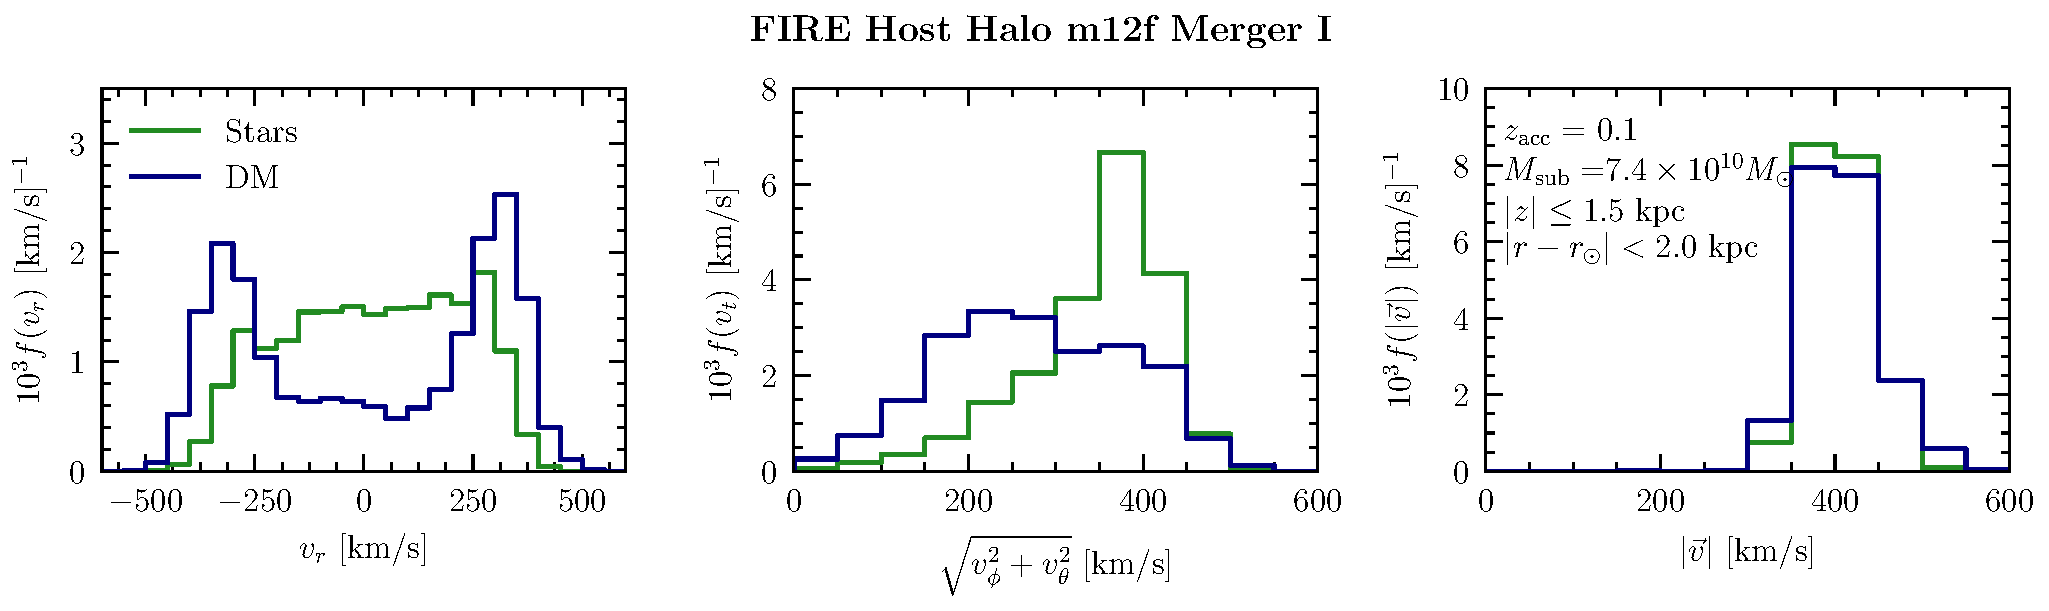
\includegraphics[width=0.95\textwidth]{plots/star_dm_vr_vt_v_merger_0m12f.pdf} 
	\qquad
	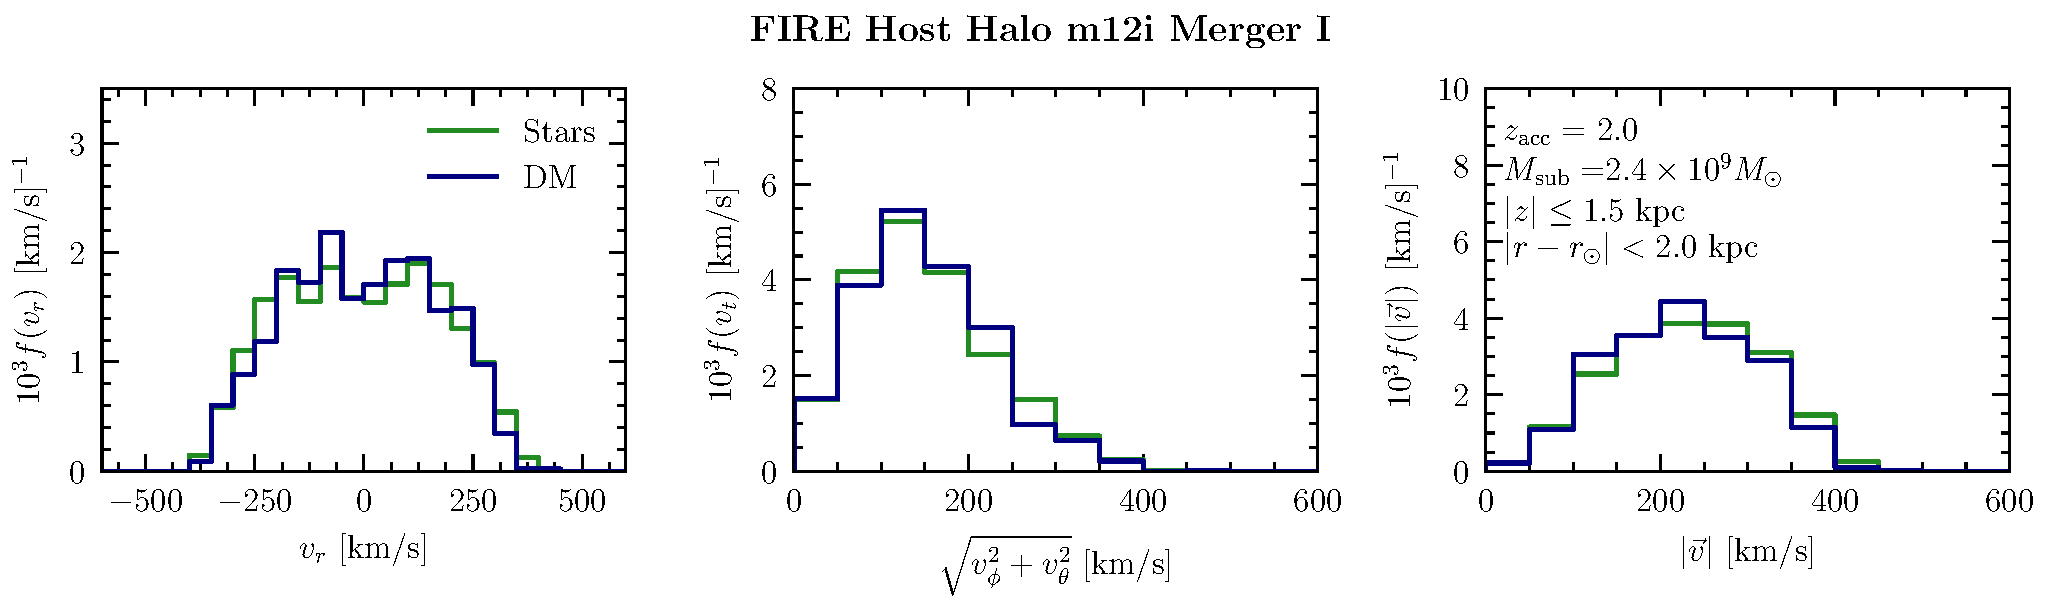
\includegraphics[width=0.95\textwidth]{plots/star_dm_vr_vt_v_merger_0m12i.pdf} 
   \caption{Velocity distributions for the debris of the largest merger in \texttt{m12f} (top) and \texttt{m12i} (bottom) that falls within the local volume, defined as $|r-r_\odot| < 2$~kpc and $|z| \leq 1.5$~kpc.  The radial (left), tangential (middle), and speed (right) distributions are shown for the stars (green line) and dark matter (blue line).  We assume a spherical galactocentric coordinate system with $\phi$ the azimuthal direction aligned with the disk rotation.  The tangential velocity is therefore $v_t = \left( v_\theta^2 + v_\phi^2\right)^{1/2}$.  The \texttt{m12i} merger is older, with $\zacc = 2$ compared to $\zacc = 0.1$.  The latter is an example of debris flow, while the former is an example of a stream.  The corresponding distributions for the other mergers listed in \Tab{tab:progenitors} are provided in the Appendix and show the same general trends. }
   \label{fig:streamdebris}
\end{figure*}



\begin{figure*}[tb] %  figure placement: here, top, bottom, or page
   \centering
	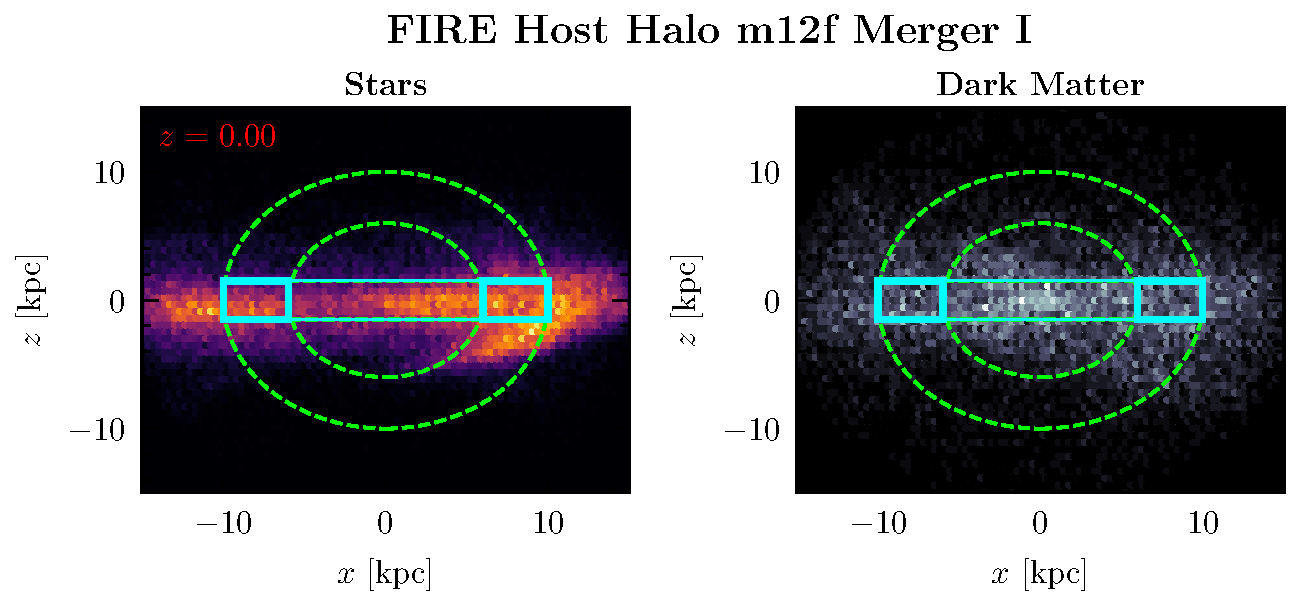
\includegraphics[width=0.75\textwidth]{plots/star_dm_position_xzxz_merger_0_snap_600m12f.pdf} 
	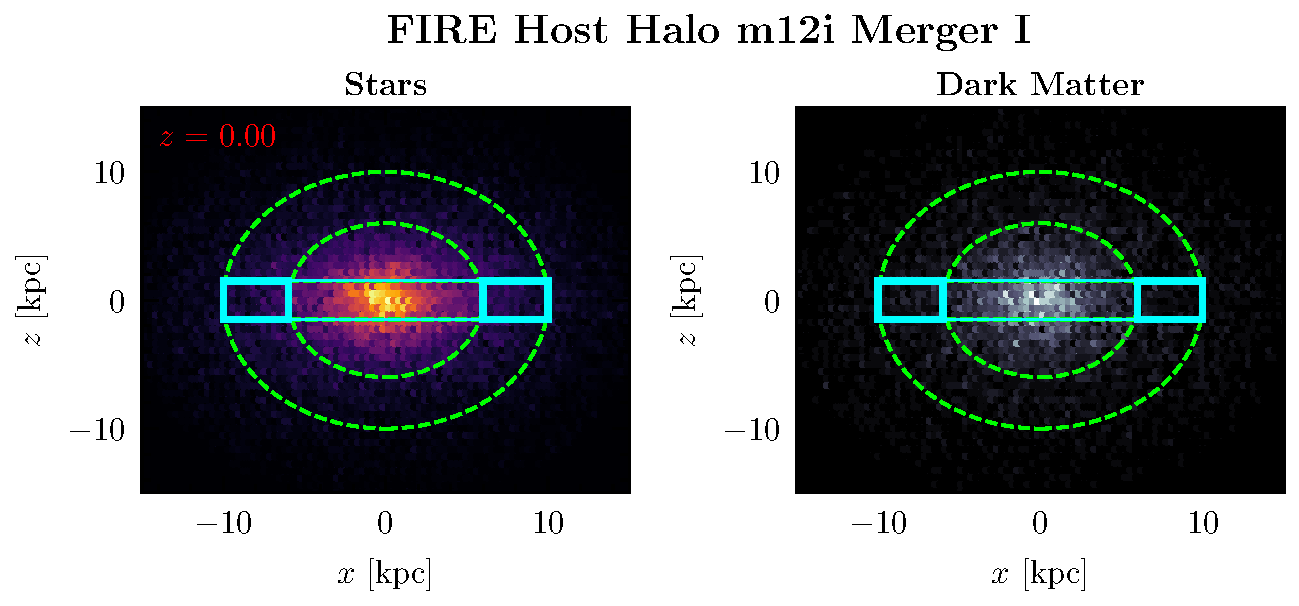
\includegraphics[width=0.75\textwidth]{plots/star_dm_position_xzxz_merger_0_snap_600m12i.pdf} 
   \caption{Density plots of stars and DM in the $x-z$ plane of the largest merger of \mf~ (top) and \mi~ (bottom). The dashed circles and rectangle show the different selection of the ROI, where the solid blue lines are the final ROI corresponding to $|z|< 1.5$ kpc, and $|r-r_{\odot}| < 2$ kpc.}
   \label{fig:position_merger}
\end{figure*}


\section{Correlation of Accreted Stars and Dark Matter}
\label{sec:correlation}

The phase-space distribution of the DM and stellar halo in the local volume is intimately linked with the galaxy's accretion history.  DM and stars that accreted onto the host at early epochs are adequately phase mixed.  More recent accretion events, however, continue to build up the mass profile of the halo.  Their debris is not fully phase mixed and can therefore be identified as substructure in either position or velocity space. In this section, 
we explore in detail the phase-space evolution of DM and stellar debris from mergers in \mi~and \mf.  We systematically study the contributions to the local volume, starting from the youngest to the oldest accreted material.  In this way, we will see how the velocity distribution of the stellar halo is built up as a function of time, and how well it traces the DM halo as the two evolve and grow together.  Host halo \mf~provides a contrasting example to \mi, as its merger history is more active up until redshifts $\sim0.1$. 
 
We emphasize that the results of this section pertain specifically to DM that is sourced by luminous satellites, \ML{would like to discuss following phrase} we define as subhalos that have contributed stars to the ROI. Most of these subhalos have total masses above $\gtrsim 10^8$~M$_{\odot}$, or stellar mass $\gtrsim 10^5$~M$_{\odot}$.  Below this mass cutoff, it is challenging to resolve a sufficient number of stars in each subhalo because the minimum mass of a star particle is $\sim 7.7 \times 10^3$~M$_{\odot}$.  The distribution of DM from the lower-mass subhalos is discussed in \Sec{sec:untracked}. 

\subsection{Substructure Component}
\label{sec:debris}

\begin{figure*}[tb] %  figure placement: here, top, bottom, or page
   \centering
	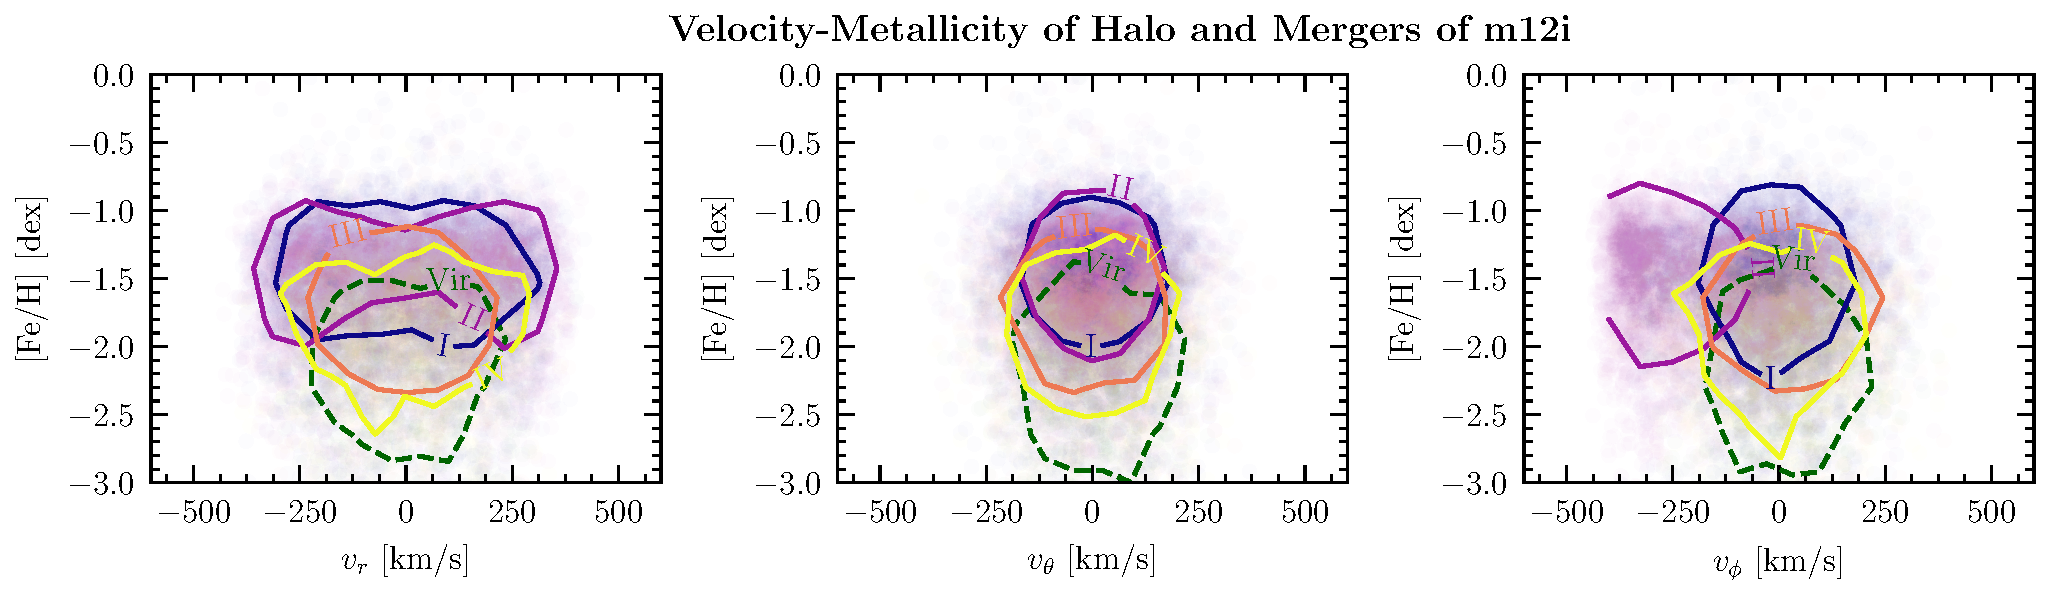
\includegraphics[width=0.95\textwidth]{plots/v_feh_mergersm12i.pdf} 
	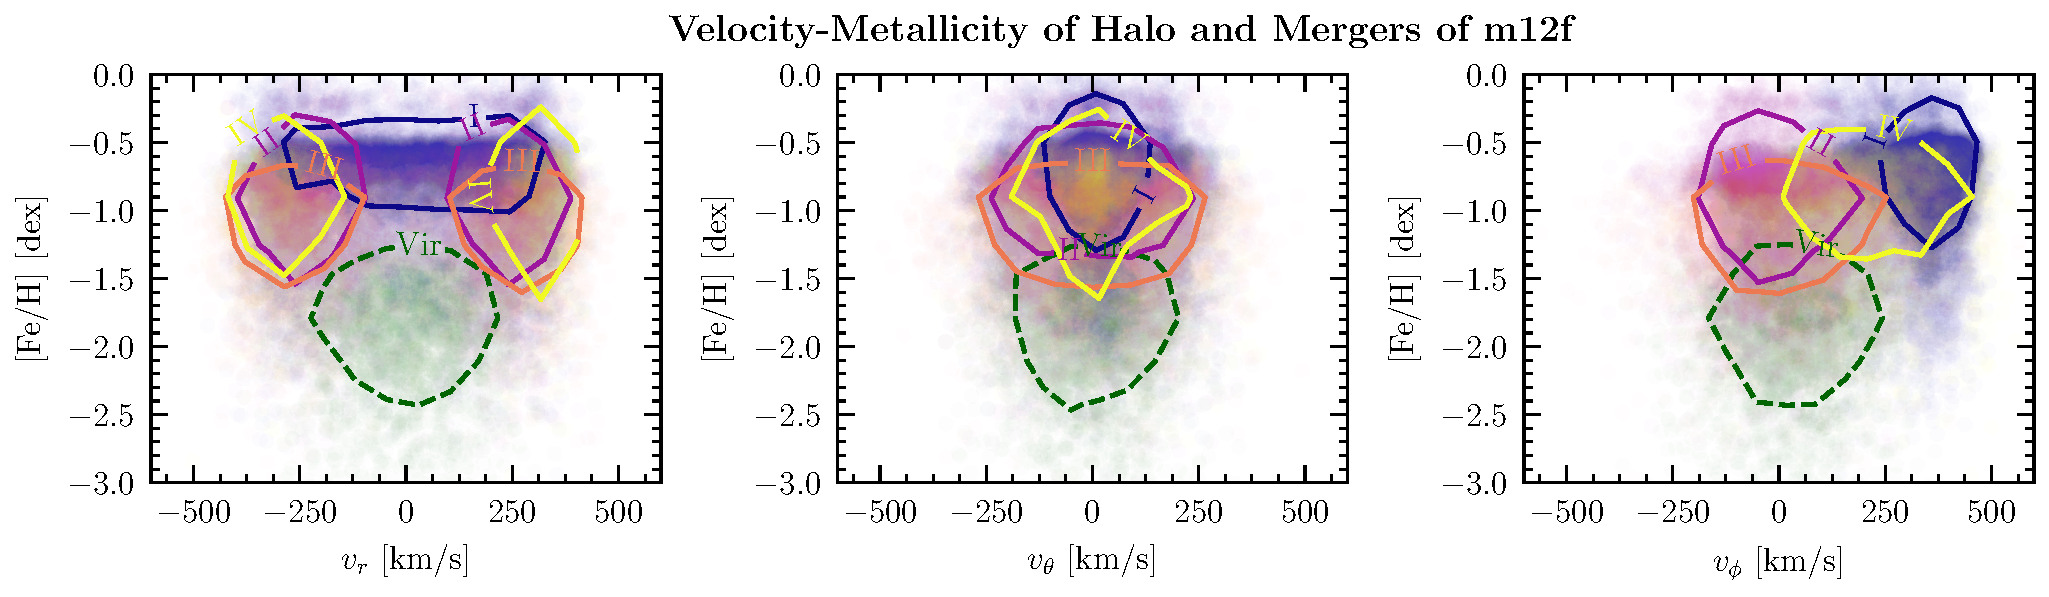
\includegraphics[width=0.95\textwidth]{plots/v_feh_mergersm12f.pdf} 
   \caption{1$\sigma$ contours in metallicity-velocity space for the four largest mergers contributing tidal debris in the local volume (blue, purple, orange and yellow solid lines), as well as the virialized component (green dashed line) of \mi~(top row) and \mf~(bottom row).   The virialized component is defined as the population of stars originating from satellite galaxies with mass $>10^8$~M$_\odot$ that were accreted before $\zacc \gtrsim 3$.  Properties of the four largest mergers are provided in \Tab{tab:progenitors}.}
   \label{fig:all_mergers}
\end{figure*}

As a satellite falls into a host galaxy, it is disrupted by tidal forces.  Depending on the accretion time, the debris either exhibits substructure in the form of streams or debris flow, or it is virialized.  When the time $t$ since accretion is on the order of the dynamical time of the system ($t\sim t_\mathrm{dyn}$),  the remains of a disrupted satellite is not well-mixed either spatially or kinematically and manifests as a stream, a structure with one-dimensional spatial morphology that is dynamically cold.   Stellar streams have been observed throughout the Milky Way halo---see~\cite{2016ASSL..420...87G} and references therein---with the best example coming from Sagittarius~\citep{Ivezic:2000ua, Yanny:2000ty}.  DM streams have been studied in numerous $N$-body simulations~\citep{Zemp:2008gw, Vogelsberger:2008qb, Diemand:2008in,Kuhlen:2009vh,Maciejewski:2010gz,2011MNRAS.413.1419V, Elahi:2011dy}. 

The most significant merger in the local volume of \mf~leaves behind a stream.  The radial, tangential, and speed distributions of the stream associated with this $6\times10^8$~M$_\odot$ subhalo accreted at $\zacc = 0.1$ is shown in the top row of \Fig{fig:streamdebris}.  The stellar distribution (green) is broad in the radial direction, while its tangential component is peaked at $v_t \sim 400$~km/s.  In contrast, the DM distribution (blue) is peaked at $v_r \sim \pm 300$~km/s, but has a broad tangential distribution.  At first glance, the DM and stellar distributions seem  uncorrelated, but the speed distribution indicates otherwise.  In particular, we see that the radial and tangential velocities of both the DM and stars conspire to yield speeds narrowly peaked about $v \sim 400$~km/s.  The small dispersion of $\sim 40$ km/s in speed suggests that the the DM and stars share a common origin in a single progenitor. 

The kinematic features of a satellite's tidal debris is linked with its orbit at the time of stripping.  For example, debris whose radial distribution is peaked was likely removed while the satellite was on a radial trajectory, falling directly into or away from the center of the galaxy.  A peak in the tangential distribution suggests that the debris was removed near the orbit's peri- or apocenter.  The differences between the distribution of DM and stellar debris in the top row of \Fig{fig:streamdebris} suggests that they were stripped at different points along the satellite's orbit.
This is further substantiated by looking at the spatial distribution of the debris.  As shown in \Fig{fig:position_merger}, the DM and stars are localized in different parts of the galaxy.  Because the debris is fairly young, it has not mixed spatially and we therefore still see the distinct points where the DM and stars were stripped along different points of the orbit.  This is expected as the stars are more tightly bound towards the center of a satellite galaxy, as compared to DM, and therefore require stronger tidal forces to be torn off.  
The fact that stellar and DM streams may not trace each other precisely was already noted in simulations of the Sagittarius stream~\citep{2012JCAP...08..027P}. 



As time proceeds ($t > t_\mathrm{dyn}$), the merger debris becomes spatially mixed but the velocity substructure persists~\citep{Helmi:1999ks} and is referred to as debris flow~\citep{Lisanti:2011as, Kuhlen:2012fz, Lisanti:2014dva}.  One can think of debris flow as the overlap of many cold streams, whose sum is dynamically hotter than any individual contribution.  Debris flow is therefore the intermediate state of tidal debris before it becomes fully mixed with the host halo at $t\gg t_\mathrm{dyn}$.  
The bottom panel of \Fig{fig:streamdebris} shows the velocity distributions of the largest merger in \mi. This $2\times10^9$~M$_\odot$ subhalo was accreted at $\zacc \sim2$, and is therefore older than the largest merger in \mf~discussed above.  In this case, the DM and stars trace each other closely in all velocity components. Most deviations between the distributions are under $10\%$, with a few up to $20\%.$

The DM and stellar debris from this merger is spatially uniform, as shown in \Fig{fig:position_merger} but its velocity distribution still retains important features that correspond to the orbital properties.  For example, the radial velocity distribution is `boxy,' a distinctive feature of satellites that are falling in radially near the local volume.  In such cases, most of the debris is stripped as the satellite moves towards/away from the galactic center, resulting in two peaks of same radial speed, but opposite direction ($\pm v_r$).  If the dispersion of these peaks is considerably larger than $v_r$, then they bleed into each other, forming a `boxy' distribution.  The fact that this velocity structure is not accompanied by spatial features---at least within the local volume considered here---suggests that it is a manifestation of debris flow.  

\begin{figure*}[tb] %  figure placement: here, top, bottom, or page
   \centering
	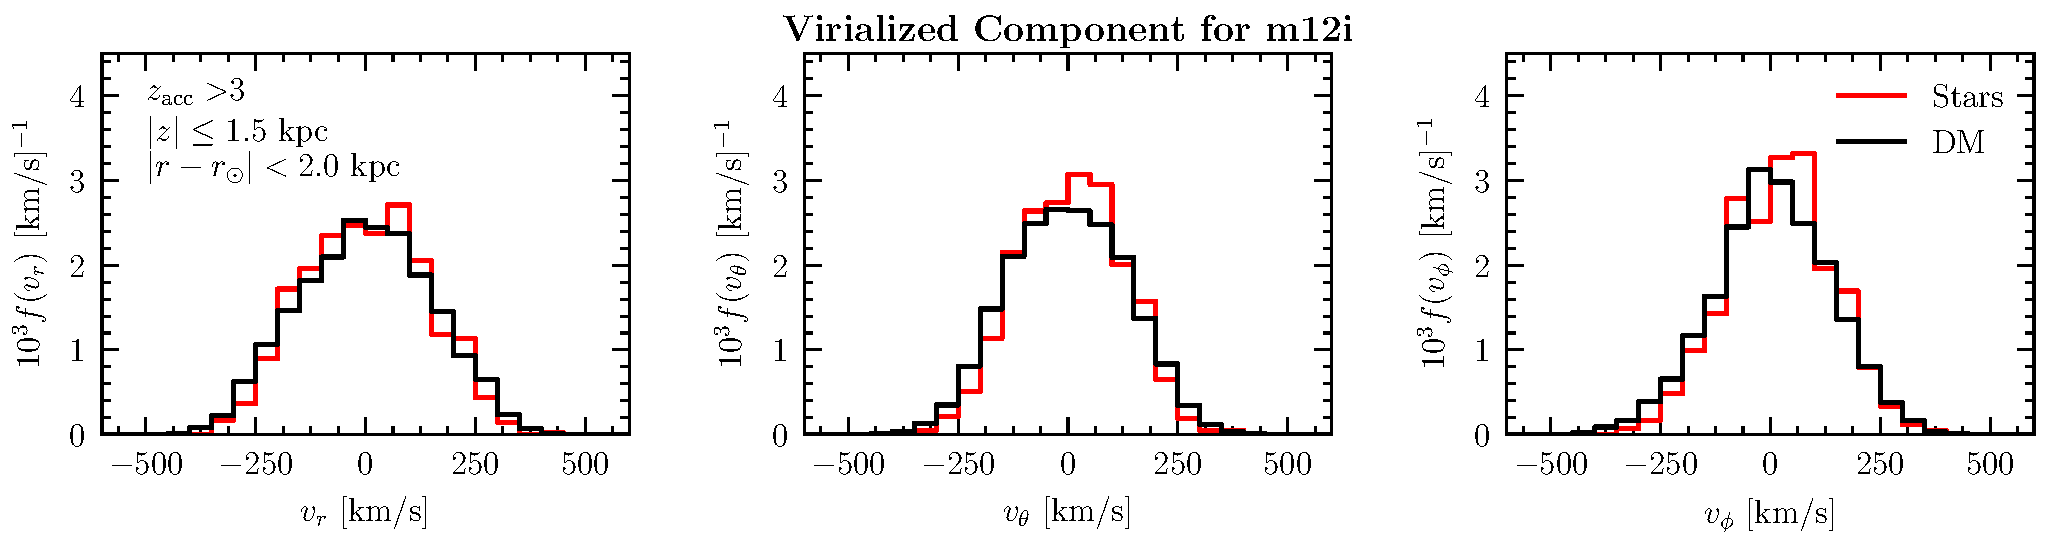
\includegraphics[width=0.95\textwidth]{plots/virialized_component_vr_vtheta_vphi3m12i.pdf} 
   \caption{Velocity distributions of accreted stars and DM in \mi~from subhalos with $z_{\rm{acc}} > 3$.  The corresponding results for \mf~are similar and are provided in the Appendix as \Fig{fig:virialized_m12f}.}
   \label{fig:virialized}
\end{figure*}


For both \mi~and \mf, the speed distributions of the stars and DM are well-correlated.  The interesting difference is that the velocity of \mf~is peaked at $\sim$$400$~km/s with a very small dispersion, while that of \mi~is peaked at lower speeds of $\sim$$250$~km/s, with a larger dispersion of $85\%$ km/s. These results indicate that the merger event of \mf~is more recent, which is consistent with what we know of its accretion time.  In general, the dispersion of the speed distribution can be an indicator for the time of the merger, with narrow dispersions pointing to a more recent origin.  

While \Fig{fig:streamdebris} only shows the distributions of the largest mergers in \mi~and \mf, we have also made the corresponding plots for the next top-three mergers contributing debris in the local volume.  These distributions are provided in the Appendix as \Fig{fig:other_mergers}.  The overall conclusions hold as there is a strong correlation between the stellar and DM distributions for these subsequent mergers as well.

In addition to the spatial and kinematic properties of the stellar debris, its chemical abundance can provide an additional handle when identifying its progenitor.  \Fig{fig:all_mergers} illustrates how the stellar debris is clustered in metallicity-velocity space.  In particular, we show the 1$\sigma$ contours of $\FeH$ against $v_r, v_\theta, v_\phi$ for the top four satellites that contribute stellar debris in the solar circle (labeled I-IV as in \Tab{tab:progenitors}) of \mi~(top row) and \mf~(bottom row).  The most significant mergers in \mi~are typically more metal-poor than those in \mf.  In particular, the average metallicity of I-IV range from $\langle \FeH \rangle \sim -1.97$ to $-1.54 $ in \mi, whereas those for \mf~vary from $\langle \FeH \rangle \sim-1.17$ to $-0.79$. This is due to the fact that the mergers contributing the most stars in \mf~occurred much later than those in \mi, as shown in \Fig{fig:origins}.  %\ML{don't understand following sentence...} Narrower distributions in metallicities might also be a hint for a smaller mass of the subhalo, where there is a smaller variation in the stellar populations, as exemplified by Merger Sr in \mf.

The radial distributions in \Fig{fig:all_mergers} demonstrate the variety of kinematic features that are possible, as already noted above.  We see examples of an extended `boxy' distribution (as in I for \mi) as well as distinctive two-lobe structures (as in II of \mf).  Some mergers leave interesting features in the azimuthal velocity distributions.  For example, II in \mi~is on a highly retrograde rotation with a speed $\sim -250$~km/s. In \mf, both I and IV have non-trivial prograde rotation of $\sim 400$~km/s and $\sim 250$~km/s, respectively.  This information, coupled with the debris' chemical abundance, is useful in determining the accretion time as well as the dynamics of the orbit.  

%These example shows the possible diversity of debris flow, and it might affect non only the speed distribution of direct detection experiments, but also any modulation signals, similarly to streams, due to anisotropic signals \citep{2012JCAP...08..027P}.


\subsection{The Virialized Component}
\label{sec:virialized}

Tidal debris from a galaxy's oldest mergers should reach dynamic equilibrium with the host.  This population is fully mixed in phase space with no distinctive features in its spatial or velocity distribution.  %\cite{Herzog-Arbeitman:2017fte} demonstrated that halo stars serve as excellent tracers for the corresponding DM using the \texttt{Eris} hydrodynamic simulation.  Here, we study this correspondence in detail for \texttt{Fire}.  Unlike in the \texttt{Eris} study, we now identify the progenitor of each star and DM particle in the solar neighborhood today, and track  
Here, we study the present-day distribution of stars and DM that were stripped from the earliest mergers in \texttt{Fire}.  Specifically, we focus on the tidal debris from satellites accreted at $\zacc >3$.  This redshift cutoff was chosen to be greater than the oldest merger that contributed more than $5\%$ of the stellar mass in the ROI---see Table \ref{tab:progenitors}.

Let us begin by focusing on the old stellar debris.  There are 23 mergers that contribute to this population in \mi, and 22 for \mf.  The average metallicity of these stars is  $\langle \rm{[Fe/H]} \rangle_{\rm{m12i}}  = -2.27$ with spread of 0.57 dex, while that of \mf~is $\langle \rm{[Fe/H]} \rangle_{\rm{m12f}}  = -1.96$ with spread of 0.50 dex. They are indicated by the green dashed region in \Fig{fig:all_mergers}, from which it is apparent that this older population is in general more metal-poor than any of the recent mergers discussed in the previous subsection.

The velocity distribution of this old stellar debris in \mi~ is shown by the red lines in \Fig{fig:virialized}.  The distributions are approximately isotropic in spherical coordinates.  Fitting the results with a multivariate distribution, we find that the dispersions are in spherical coordinates $\{ \sigma_r, \sigma_{\theta}, \sigma_{\phi} \} =  \{138, 119, 121 \}$ km/s. These dispersions are close to being isotropic, which is expected of the virialized component. This also indirectly justifies our choice of the virialization cutoff of $z_{\rm{acc}}=3$.

Next, we compare the stellar distributions with that of the DM debris from the same mergers, shown by the black line in 
\Fig{fig:virialized}.  Notably, both the stellar and DM distributions trace each other closely. We find that the discrepancies between the distributions are between $3\% $ and $25\%$, which gets amplified to $\sim 40\%$ at the tails. 

The spatial distributions associated with the virialized component do not show any spatial features for both the DM and the stars, which is consistent with the near isotropic velocity distributions of both distributions.

It is worth emphasizing that the correspondence between DM and stars is non-trivial, as each merger might contribute a different stellar fraction to dark fraction, and we are summing over all 23 mergers here.  This is due to the fact that all these distributions have long been virialized, and therefore are close to being just isotropic in spherical coordinates. Summing over different mergers with similar distributions, although they contribute different amounts of DM and stars, leads to the same total distribution and the excellent agreement between the stars and the DM.

Before concluding, we note that the results of this section remain the same for a Milky Way--like halo with a more active merger history, as in the case of \mf--see \Fig{fig:virialized_m12f} in the Appendix.


\section{The Total Dark Matter Distribution}
\label{sec:totaldarkmatter}

\begin{figure*}[tb] %  figure placement: here, top, bottom, or page
   \centering
	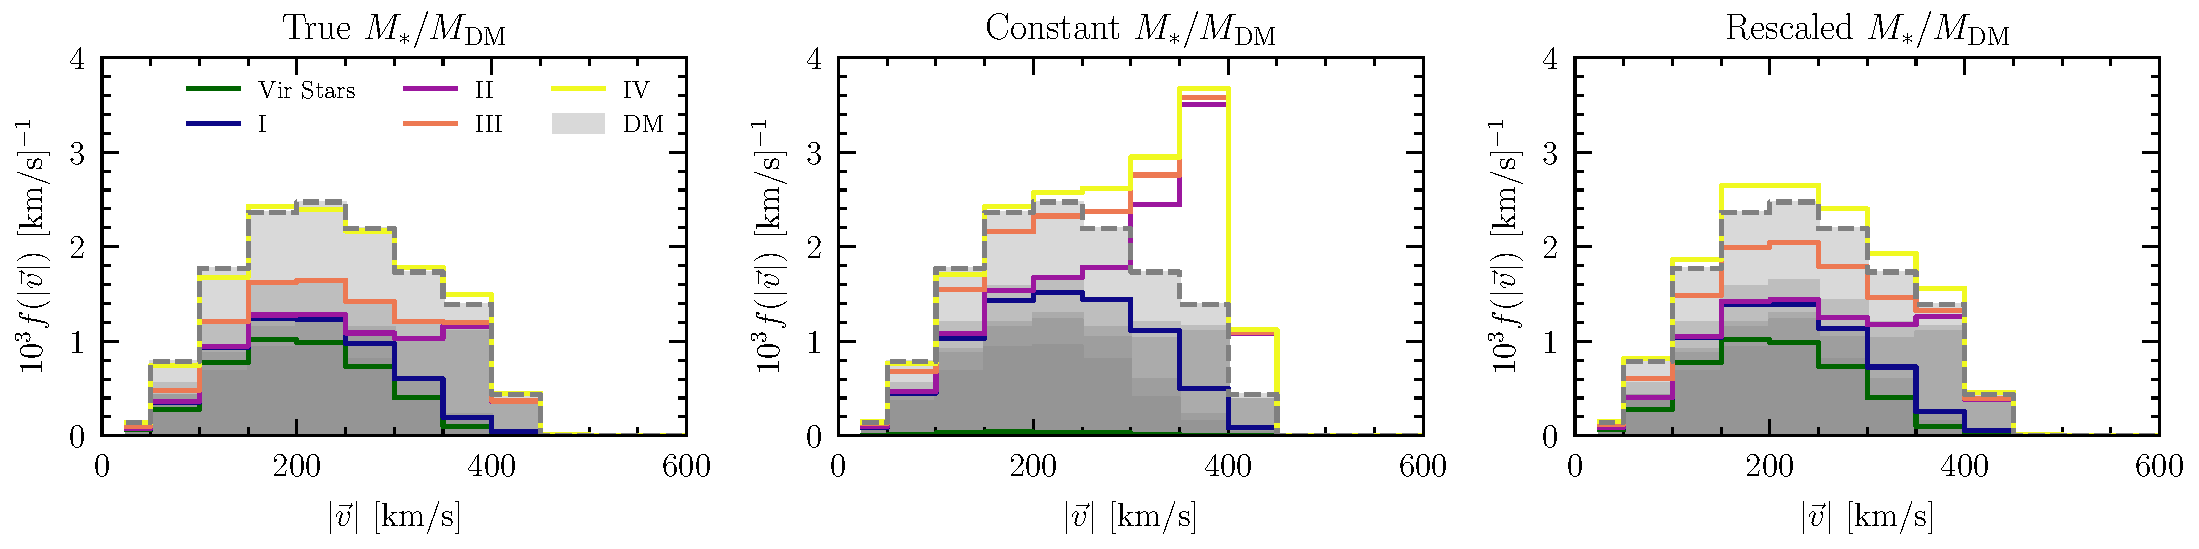
\includegraphics[width=0.95\textwidth]{plots/construct_dm_from_stars_m12i.pdf}
   \caption{Building the DM distribution from the stellar distributions. The gray distribution in all three panels is that of DM accreted from luminous satellites. (Left) The stacked stellar distribution of the virialized component, as well the speed distributions of the four most dominant mergers in stellar mass, and all other mergers are shown. These distributions are those of the stellar component, scaled as though each merger contributed an equal number of stars and DM. (Middle) The stacked stellar distribution of the virialized component, as well the speed distributions of the four most dominant mergers in stellar mass, and all other mergers are shown. However, these distributions are scaled by their stellar mass contribution to the ROI. (Right) The stacked stellar distribution of the virialized component, as well the speed distributions of the four most dominant mergers in stellar mass are shown, from the scaling relation given by \Eq{eq:scaling_relation}. Other mergers are not shown due to selection effects (see discussion in the text). }
   \label{fig:rescaling}
\end{figure*}

In the previous section, we saw that the kinematics of the DM and stars that are accreted from luminous satellites are well-correlated, at least in the case of the old virialized component and debris flow.  Now, we study how one can add up the contributions from the separate mergers to build the total dark matter distribution in the local volume.  In Sec.~\ref{sec:luminous}, we demonstrate how to combine the contributions of DM that is sourced from luminous satellites, focusing on the old virialized populations and substructure from additional large mergers.  In Sec.~\ref{sec:untracked}, we turn to the population of DM that is not traced by the stars---that is, the component from dark subhalos and smooth accretion.

\subsection{Component from Luminous Satellites}
\label{sec:luminous}

Here, we will focus on how to build the total DM distribution once one has individually characterized the kinematics of the virialized stellar halo as well as additional velocity substructure.  As we have seen, when each of these components is considered in isolation, the DM and stars successfully trace each other.  However, more realistically, a halo is formed from the combination of more than one of these components and we must understand how the two can be added together.    
  
To introduce the challenges associated with such a combination, let us try to build the DM speed distribution from that of the stars using several different procedures.  Consider the left-most panel of \Fig{fig:rescaling}.  The ``true" DM distribution in the local volume that is sourced be the virialized subhalos as well as the top four largest mergers that were discussed in \Tab{tab:progenitors} is shown by the filled histogram in gray. The colored lines show the \emph{stacked} contributions from the corresponding populations of stellar debris that contribute to the local volume. To emphasize, we are plotting the stellar distributions, not the DM ones. The first histogram (green) is that of the virialized component, which includes stars from the mergers with $\zacc > 3$, whereas the next four histograms (blue, purple, orange, and yellow) represent the additional contributions from mergers I-IV in \mi.  When stacking the contribution of the different stellar components, we weigh their contribution by the fraction of DM contributed by the merger, relative to that of the virialized population.  This ratio would be unity if mergers I-IV each contributed the same amount of DM to the local volume compared to the virialized component.  This is not the case, however; the exact weights with respect to the virialized component that we find are $\{0.29, 0.44, 0.38, 0.91 \}$.  As we see from \Fig{fig:rescaling} (left), the procedure described above reproduces the total DM distribution.  Of course, this is to be expected given that we have already demonstrated the correspondence for each separate population and have simply taken their DM fraction from the simulation.  
%We stack the distributions of the stellar merger over the virialized component, scaling them by their relative DM contribution, and finally we show in orange the following smaller mergers, similarly scaled. During this process, we have effectively assumed that all stellar components contribute an equal number of stars as DM.   scaled by their contributions in DM: , and scaled them by the relative fraction of the virialized DM to the total DM distribution
%\ML{I'm assuming for the moment that we won't be showing the contributions from the orange guys...}
%The final stacked speed distribution of the stars is closely correlated with that of DM. The reason the correlation is not as strong as the one from Figs.  \ref{fig:stream}, \ref{fig:debris_flow}, and \ref{fig:virialized} is due to mergers with very few stars, where the distributions are not smooth. In the infinite particle limit, this problem should be resolved.

\begin{figure*}[tb] %  figure placement: here, top, bottom, or page
   \centering
	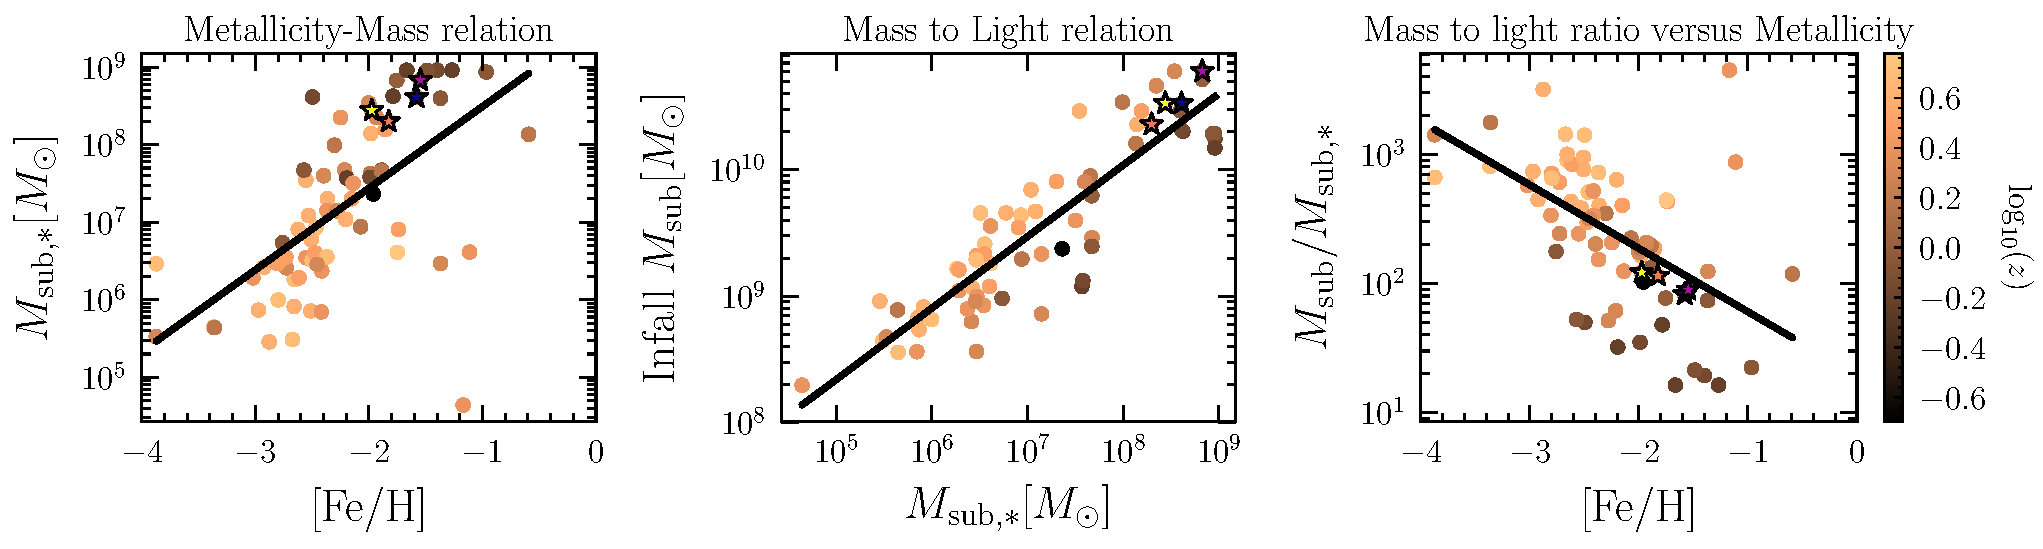
\includegraphics[width=0.95\textwidth]{plots/feh_infall_mass_ratios_all_subhalos_m12i.pdf}
   \caption{(Left) Metallicity-Mass relation of the subhalos contributing stars to the ROI. The colored dots are of the four most dominant mergers, matching the same color convention in Figs \ref{fig:all_mergers} and \ref{fig:rescaling}.  (Middle) Mass to light relation of the different subhalos in the ROI. (Right) Ratio of subhalo mass to the subhalo stellar mass as a function of the average metallicity of each subhalo.}
   \label{fig:scaling_relation}
\end{figure*}


In actuality, of course, one does not precisely know the DM contribution that is associated with the merger---observations only provide the relative stellar fraction of each contribution.  In the middle panel of \Fig{fig:rescaling}, we show what happens when each contribution is weighted by its    
relative stellar fraction instead.  In this case, the final stacked distribution is quite different from the DM one.  This is because the largest mergers dominate the stellar distribution more-so than they dominate the DM one (as seen in the first panel). First, the contribution of the virialized component to the stellar halo is $0.5\%$ of the total \emph{accreted} stellar mass in the ROI while the virialized DM is $11 \%$ off the total \emph{accreted} DM mass in the ROI. In subsequent mergers, the stellar fractions are given by \Tab{tab:progenitors}, or as a fraction of the virialized DM component (so it can be compared to the numbers above) $\{ 2.84, 2.66, 1.31, 0.59 \}$.

As a result, we need a more sophisticated algorithm for inferring the amount of DM that is contributed by each stellar population.  Such an extrapolation is indeed possible using the metallicity-mass relation and mass-to-light ratio.  Combining these two relations, one can use the observed metallicity to infer the mass-to-light ratio of a satellite progenitor.   We will now illustrate this procedure in detail for \mi.  

The left and middle panels of \Fig{fig:scaling_relation} show the metallicity-mass relation and mass-to-light ratio for \mi, respectively.  We only plot the subhalos that contribute tidal debris within the local volume\ML{Kirby relation would apply to all subhalos}.\footnote{Technically, since rockstar was only run on the DM particles, the subhalo mass shown here is that of the DM only. In most cases the stellar contribution is much smaller, so the total subhalo mass is dominated by the DM mass, however this is not true for all mergers.} 

Performing a linear fit yields the following two relations:
\be \label{eq:metallicity_mass}
\log_{10}(M_{\rm{sub}, *}) = 9.16 + 0.96 \langle \rm{[Fe/H]} \rangle,
\ee 
and 
\be \label{eq:mass_to_light}
\log_{10}(M_{\rm{sub}}) = 4.5 + 0.68 \log_{10}(M_{\rm{sub}, *}) .
\ee
Combining Eqs.~\ref{eq:metallicity_mass} and~\ref{eq:mass_to_light} yields
\be \label{eq:ratio_relation}
\log_{10} \left(\frac{M_{\rm{sub}}}{M_{\rm{sub}, *}} \right) =1.57-0.31 \langle \rm{[Fe/H]} \rangle \, ,
\ee
which only depends on the previous fit parameters.  In this way, one can derive the dependence of the mass-to-light ratio on the stellar metallicity.  

While this is the procedure that one would follow in practice for the Milky Way, we can also obtain this relation exactly when working with the simulation.  For example, the right panel of \Fig{fig:scaling_relation} plots the ratio $M_{\rm{sub}}/M_{\rm{sub}, *}$ as a function of the observable mean metallicity in \mi, and is well-fit by 
\be \label{eq:scaling_relation}
\log_{10} \left( \frac{M_{\rm{sub}}}{M_{\rm{sub}, *}} \right) = 1.47 - 0.37 \langle \rm{ [Fe/H] } \rangle,
\ee
which is consistent with the relation derived as \Eq{eq:ratio_relation}.
Mergers I-IV are indicated by the colored stars in all panels of \Fig{fig:scaling_relation}.  Using Eq.~\ref{eq:scaling_relation}, we would infer their mass-to-light ratios to be $\{ 116, 111, 154, 180 \}$ which are close to their true values $\{82, 89, 115, 122\}$ respectively. These small discrepancies are due to the scatter in \Fig{fig:scaling_relation}.

We can now use the inferred mass-to-light ratio to re-weigh the contributions of the separate mergers in \mi.  To start, we use the average metallicity of the virialized stellar halo (as given in  \Sec{sec:virialized}) in \Eq{eq:scaling_relation} to obtain the ratio $\log(M_{\rm{sub}}/M_{\rm{sub}, *})_{\rm{halo}}$.  We find the ratio of the subhalo DM mass to the stellar mass $(M_{\rm{sub}}/M_{\rm{sub}, *})_{\rm{Merger}}$  divided by that of the halo $(M_{\rm{sub}}/M_{\rm{sub}, *})_{\rm{halo}}$ to be $\{0.11, 0.10, 0.14, 0.17 \}$ , which compares well to the exact value of $\{0.07, 0.10, 0.09, 0.21\}$.  We then repeat this procedure for mergers I-IV, and rescale the histograms by these values.  The results are shown in the third panel of \Fig{fig:rescaling}.  Comparing this with the first panel, we find that we recover the DM contribution of the most dominant mergers correctly. This gets up a step closer to the full reconstruction of the DM speed distribution.   

In \Fig{fig:constructed_dm}, we apply the same procedure to \mf, which has a more active merger history, and find that we can indeed recover the DM speed distribution of the virialized component and the top few mergers correctly. This might be somewhat surprising as the largest merger of \mf~is a stream as has been discussed in \Sec{sec:debris}. We have shown in \Fig{fig:streamdebris} that although the stars do not trace the component distributions of the velocities of the DM, they do trace the speed distribution, which is plotted in  \Fig{fig:constructed_dm}. 

We have successfully rescaled the speed distributions of the stars to obtain that of the DM for the top mergers, however, we did not rescale all subsequent smaller mergers. The reason is that doing so ends up over shooting the contribution. This is due to two issues: selection effects and the presence of streams. The first is a simulation issue that can be side-stepped while analyzing the Milky Way, while the second cannot. 

Selection effects are due to subsampling small subhalos. For large mergers, sampling them along the ROI is sufficient to obtain more or less the correct ratio of stars to DM. For smaller mergers, however, sampling in a small area such as the ROI can lead us to getting only one or two star particles with a lot more of the DM, if one starts with a handful of particles. This is not an issue in the Milky Way as there should not be a resolution threshold to low mass luminous satellites, or at least, such satellites have a negligible contribution to DM from luminous satellites.

As argued in \Sec{sec:debris}, in the case of streams, one can find spatial offsets between the DM and the stars, as shown by \Fig{fig:position_merger} . Such offsets can be affected by the selection of an ROI as one might oversample the DM compared to the stars, since the stars are usually more tightly bound, while the DM can extend further.  Reproducing the contribution of these smaller subhalos will be the object of future work.

%In order to side-step issue, we attempt to reproducing the DM that has merged at $z > 1$. This avoids all small stream contamination. We find an excellent agreement between the rescaled velocity distributions of the top 4 mergers in \Fig{fig:constructed_dm} and the DM from $z>1$. We see an equivalently excellent agreement for \mf~that we show in the appendix as \ref{fig:constructed_dm_mf} with the two non-stream mergers. 

\begin{figure}[tb] %  figure placement: here, top, bottom, or page
   \centering
	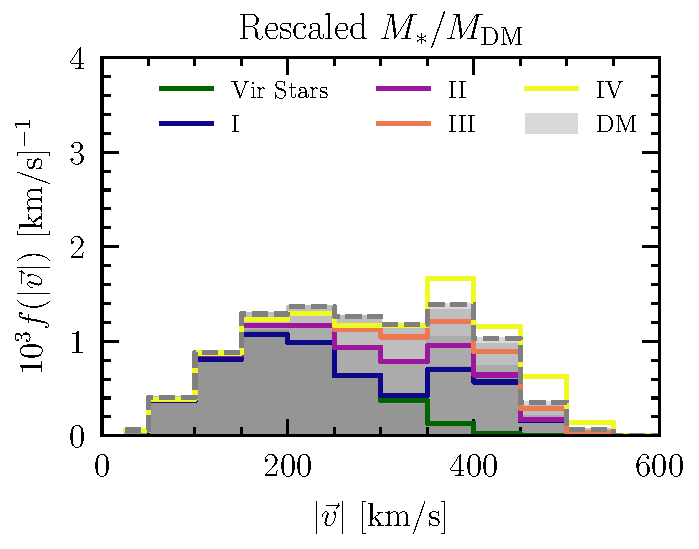
\includegraphics[width=0.45\textwidth]{plots/construct_dm_from_stars_top_mergers_m12f.pdf}
   \caption{Reconstructing the DM distribution using the velocity distributions of the virialized component and the largest mergers in \mf. This is equivalent to the last panel of \Fig{fig:rescaling}}
   \label{fig:constructed_dm}
\end{figure}


\subsection{Untracked component}
\label{sec:untracked}




Although we found an excellent correlation between the velocity distributions of the stars and the DM from the largest luminous satellites, and succeeded at rescaling the stellar contribution to match that of the DM,  we need to address the DM contribution from non luminous satellites. Such a contribution is usually sourced through smooth accretion, where the DM is merging into the Milky Way without being previously associated with a subhalo, and through dark subhalos where subhalos usually of masses smaller than $\sim 10^8 M_\odot$, and did not form stars (above the simulation's resolution).


\begin{figure*}[tb] %  figure placement: here, top, bottom, or page
   \centering
	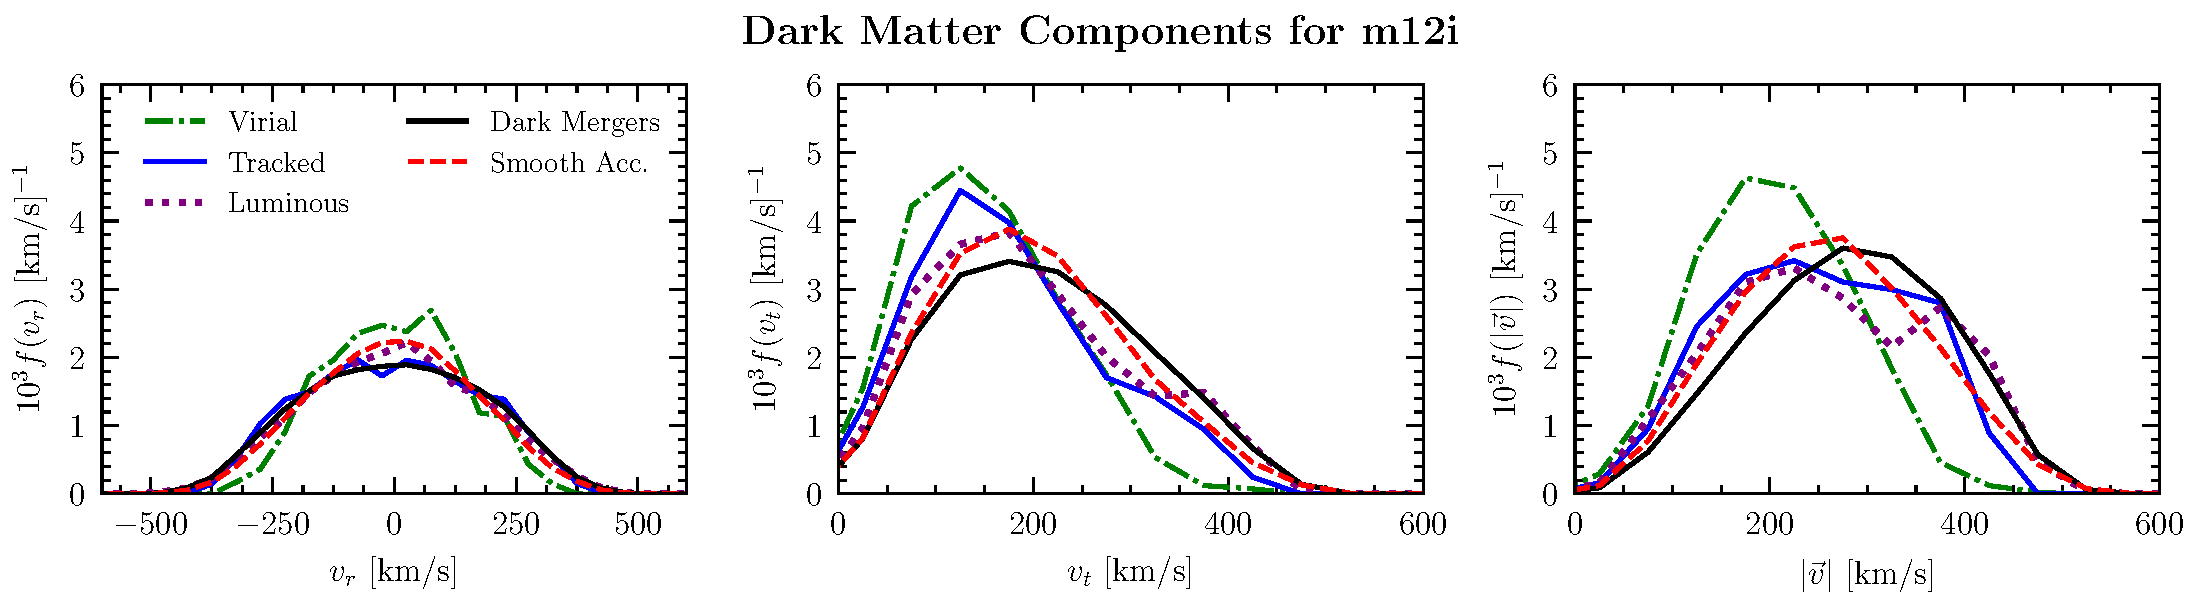
\includegraphics[width=7in]{plots/untracked_compoenents_m12i.pdf}
	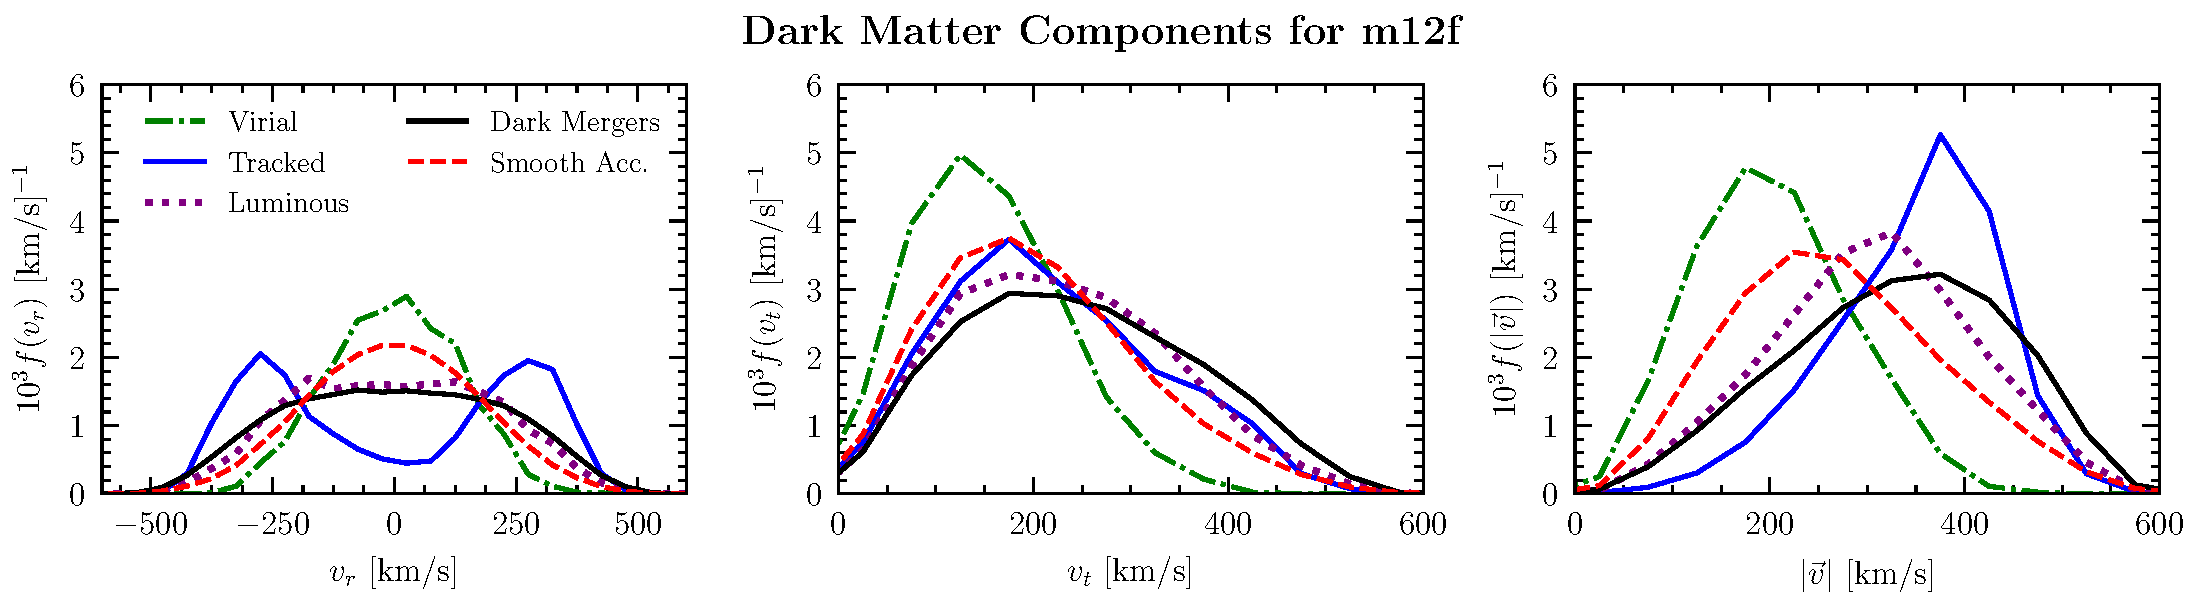
\includegraphics[width=7in]{plots/untracked_compoenents_m12f.pdf} 
   \caption{Velocity distributions of DM particles, divided by origin: we plot the virialized component (green) and the top four mergers that we label as tracked (blue). Both contributions have already been shown in \Fig{fig:rescaling}. The other components are smooth accretion (red), the luminous though smaller satellites (purple) and finally the dark mergers that do not contributed stars to the ROI.}
   \label{fig:unvirialized}
\end{figure*}


%Not all of DM can be traced through the stars, as some of the DM can have been formed through smooth accretion, or through mergers of small enough subhalos that have not formed stars. 
In \Fig{fig:unvirialized}, we show the velocity distributions $v_r, v_t$ and $|\vec{v}|$ of the virialized component, the largest four stellar mergers which we label as tracked, as well as the smoothly accreted component, DM that has been accreted by subhalos that do or do not contribute stars to the ROI, which we label luminous and dark respectively. The first two components have already been addressed in \Sec{sec:luminous}. We now study the remaining components in turn.

To identify the smoothly accreted DM component, we perform the algorithm of associating particles with subhalos, as described in \Sec{sec:origins}. All DM particles that have never been associated with a subhalo are then labeled as particles that have merged though smooth accretion. 
%We do not think that this has affected our results drastically as we could see an excellent correlation between the DM and the stars.

In \Fig{fig:unvirialized}, we show the velocity distribution of the smooth accretion, which contributes $\sim 33\%$ to the total DM in the ROI. This percentage varies greatly in each simulation, as has been shown in \cite{2011MNRAS.413.1373W}. For the case of \mi~(top panel), we find that the smooth accretion distribution does not show any specific characteristics in the $v_r$ distribution. It has a slightly larger dispersion than that of the virial distribution, which is also reflected in the speed distribution. We also find that the smooth accretion component has a tangential velocity peaked at $\sim 200$ km/s which is slightly larger than the tracked mergers which peak at $\sim 140$ km/s and the virial component, which also peaks at $\sim 140$ km/s. This leads to the speed distribution peaking at a velocity of $\sim 260$ km/s, which is larger than that of the virial component at $\sim 190$ km/s, and is somewhat comparable to that of the tracked (top four mergers) components which has a wider speed distribution. This is due to the superposition of multiple mergers of different dispersions as can be seen in \Fig{fig:other_mergers}.

The velocity distributions of \mf, shown in the bottom panel of  \Fig{fig:unvirialized} of the smooth component show a similar behavior as \mi. The same is seen of the virialized component. The largest difference between \mi~and \mf~ is that of the tracked component, as expected. \mf~has younger mergers with high speed distributions (as can be seen in \Fig{fig:streamdebris}). This leads to the ``loby" structure in the radial velocity panel, as well as the speed distribution, which dominated by its largest merger that contributes 40\% of the stellar mass (see \Tab{tab:progenitors}) has a strong peak at 400 km/s. 

Comparing the luminous component distribution between \mi~and \mf, we find that for the case of the quiet merger history, the distribution is close to that of the tracked component and the smooth accretion. This is due to the fact that these smaller subhalos are mostly in the state of debris flow, somewhat similar to the tracked component. Future study should lead to a rescaling relation in order to be able to extrapolate these distributions from the stars. For \mf, we find that there is a ``boxy" behavior and a high dispersion in $v_t$, which combines to give a speed distribution that peaks at $\sim 320$ km/s. This is consistent with the fact that mergers in \mf~are more recent and have higher speeds. 

Finally, we study the dark halo contributions to \Fig{fig:unvirialized}. We find that the dispersions in $v_r$ and $v_t$ are larger than those of the virialized component for \mi, which leads to an overall larger speed distribution, peaking at $\sim 320$ km/s for the dark mergers. These dark mergers are composed of completely dark subhalos, which are smaller subhalos that have not formed stars, of masses $\lesssim 10^8 M_{\odot}$. In both cases, this leads to somewhat smaller subhalos in size, that tend to have larger merging speeds. The same behavior can be seen in \mf, although the radial velocity distribution is boxier with a large dispersion that extends from $-250$ to 250 km/s. The dark mergers have the largest dispersion in the tangential velocity, and peak at almost $|\vec{v}| \approx 400$ km/s.

Constructing the smooth accretion and dark merger components requires further study, as they are intertwined with the merger history of the galaxy under consideration, but cannot be traced empirically using the stars. 
 
%We note however that the distribution seems close to isotropic, especially in the case of \mi, which is in the top panel of \Fig{fig:unvirialized}. This is reassuring, as one can rescale the virialized component to obtain an approximation of the contribution of the smooth accretion.
%
%In the same figure, we also show the DM from subhalos, broken up by mass of the merging subhalo. We associate the contribution of subhalos with masses larger than $10^8 M_{\odot}$ to be dominated by that of the virialized component as was shown in \Sec{sec:direct_detection}. This exercise however shows the difference in the velocity distributions between small subhalos and larger mass ones. We see for example that the low mass subhalos have larger velocity dispersions, which (as we have checked) lead to peaks in the speed distribution of $|\vec{v}| \sim 350~$km/s, while the larger masses peak at lower speeds of $\sim 200~$km/s. We also see that the radial velocity distribution of the smaller subhalos is more box-like, while that of the massive subhalos is more peaked at zero. This is a hint that a sizable number of these small subhalos are still in the stage of debris flow, and indeed we find that they contribute at later times. \lmn{Check and understand this}


\section{Building the Milky Way's Dark Matter}
\label{sec:milky_way}

Using the procedure developed in previous sections, we are now move to building the velocity distribution of DM in the Milky Way. As was shown in \Sec{sec:totaldarkmatter}, we are able to rescale the velocity distributions of the stars from the virialized component, as well as the top contributing mergers. In a recent study, \cite{necib2018} fit the velocity distributions of Gaia DR2 data \citep{2016A&A...595A...4L,2018arXiv180409365G} crossed with SDSS \citep{} to extract the stellar halo component and that of a large debris flow called the \emph{Gaia} Sausage~\citep{2018MNRAS.478..611B,2018ApJ...856L..26M,Myeong:2018kfh,2018ApJ...862L...1D,necib2018,2018arXiv180704290L} or Gaia-Enceladus \citep{2018arXiv180606038H}.  
In this study, we found the average metallicity of the Milky Way [Fe/H]$_{\rm{MW}} = -1.82$, while that of the Gaia Sausage to be [Fe/H]$_{\rm{Merger}} = -1.40$. 

Paralleling our work in \Sec{sec:luminous}, we start with the stellar-mass relation of \cite{Kirby:2013wna}, 
\be
\langle \rm{[Fe/H]} \rangle=(-1.69 \pm 0.04)+(0.30 \pm 0.02) \log_{10} \left(\frac{M_*}{10^6 M_\odot} \right).
\ee
We assume an error of 0.4 dex on the metallicity similarly to \cite{2016ApJ...821....5D}, which translates to an error of 1.3 dex in $\log_{10}(M_*)$.

Moving to the Light to Mass relation from \cite{Garrison-Kimmel:2013eoa}, we find
\be
\log_{10}(M_{\rm{peak}})= (\log_{10} (M_*) + 12.72)/1.92
\ee
Assuming 0.3 dex scatter in $\log(M_*)_{10}$ as per \cite{2016ApJ...821....5D}, we find an error of $\sim$0.16 dex on $\log_{10}(M_{\rm{peak}})$.

Putting everything together, we find
\be \label{eq:mw_rescaling}
\log_{10} \left( \frac{M_{\rm{peak}}}{M_*} \right) = 1.05 - 1.6 \langle \rm{[Fe/H]} \rangle.
\ee
Using \Eq{eq:mw_rescaling}, we can now rescale the contribution of the Sausage to that of the virialized component, and find that the velocity distribution of the substructure should contribute 
\be
a_{\rm{Merger}} = 0.23^{+1.60}_{-0.20} a_{\rm{Vir}},
\ee 
to that of the virialized component, where $a_{\rm{Merger}}$ and $a_{\rm{Vir}}$ are the normalizations of the substructure and the virialized components respectively. The error bar on the normalization is large due to the scatter of the mass to light relation, but it is a first construction of the velocity distribution from that of the stars. Its implications for direct detection are discussed in \cite{necib2018}.

\section{Conclusions}

In this paper, we built on the previous work of \cite{Herzog-Arbeitman:2017fte} which asserts that metal poor stars can be used as tracers for the velocity distribution of DM to argue that (1) stars from old virialized mergers are excellent tracers for the virialized DM component, and (2) stars from more recent mergers that leave a debris flow also trace their DM counterparts. Mergers, however, contribute different amounts of DM and stars. We have therefore shown that one could find the necessary rescaling factors when combining the mass-metallicity relation with the light to mass ratio in order to relate the ratio of subhalo peak mass to its stellar mass $M_{\rm{sub}}/M_{*}$ to an observable such as the average metallicity of a merger. With such relation, we can renormalize the contribution of each new merger to that of the virialized component, knowing its average metallicity, and successfully build the DM velocity distribution of the virialized components and the most significant mergers. 

Using the new rescaling relation has its limitations in the simulations. Subhalos that contribute very few stars, or no stars at all in the ROI, might lead to an inaccurate sampling of the ratio of the DM to stars within the ROI. This is partly due to the resolution of the simulation as the smallest stellar mass is of $\sim 7700 M_{\odot}$, and partly due to the presence of streams, where if the stream is not large enough, the selection from the ROI can be oversampling the DM at the expense of the stars.

This empirical method of inferring the DM distribution from the stars does not take into account the contributions from DM that has been smoothly accreted, or that belonging to dark subhalos. Both components, lacking stars by definitions, are harder to empirically trace. Future study is required in order to correctly extrapolate these contributions. One cannot simply take the distributions from the simulations.
\texttt{m12i} and \texttt{m12f} provide two realizations of Milky-Way--like halos that serve as interesting counterpoints in understanding the effects of different merger histories on observable DM properties.  However, it is important to keep in mind that these two examples do not fully capture all  possibilities.  Previous studies using high-resolution DM-only $N$-body simulations have found considerable variation in the potential origin of DM in the solar neighborhood.  For example, the DM halo in the \texttt{Via Lactea} simulation is rapidly built up around $z\sim 1.7$ and then remains essentially stationary until $z=0$~\citep{Diemand:2007qr}.  In some \texttt{Aquarius} halos, the DM in the solar neighborhood is nearly all in place before $z\sim6$, whereas in others, most of the DM accreted more recently~\citep{2011MNRAS.413.1373W}.  This underscores the importance of studying a variety of simulated halos to better understand how the distribution of local DM is affected by a galaxy's formation history.  Only in this way, can we robustly  extrapolate conclusions to the Milky Way.  


In a recent study, \cite{necib2018} extracted the velocity distributions of the virialized component as well as that of a large debris flow called the Gaia Sausage in the solar circle. This work provides a framework for how to correctly extract the DM distribution from that of the stars by showing that the stellar halo traces the DM virialized component, and also that the Gaia Sausage should also trace its DM counterpart. Using the rescaling relations from \Sec{sec:milky_way}, we can obtain the relative contribution in DM of the Gaia Sausage with respect to the virialized DM component, and build an empirical understanding of the velocity distribution of DM, albeit still lacking the contribution of smooth accretion and dark subhalos.



Extracting the correct DM velocity distribution plays an important role in direct detection of DM. This is the process in which a DM particle scatters off a heavy nucleus, which recoils and produces a detectable signal \citep{Goodman:1984dc}. The rate of this process depends on the speed distribution of the incoming DM. In \cite{necib2018}, we use the current findings to estimate direct detection bounds as a function of DM mass, with the empirically determined velocity distribution. We find that previous limits using the Maxwell Boltzmann distribution ~\citep{Drukier:1986tm,Freese:1987wu} are overly constraining at low DM masses. These limits can still vary largely once the dark components of DM are taken into account.

%\ML{Words regarding implications for direct detection}
%The local DM velocities are typically assumed to follow a Maxwell Boltzmann distribution, as first hypothesized  by~\cite{Drukier:1986tm,Freese:1987wu}.  This form is motivated by the fact that the Galactic rotation curve is flat near the Solar position~\citep{2012ApJ...759..131B}.  A constant circular velocity implies that the enclosed DM halo mass must scale linearly with radius, as $v_c = \sqrt{G M(r)/r}$.  This, in turn, means that the local mass density must be $\rho(r) \sim r^{-2}$, as satisfied by the singular isothermal sphere.  If we assume that the DM dominates the local mass density and is in steady state, then its velocity distribution can be inferred from Jeans Theorem---the final result is the Maxwell Boltzmann distribution.  Other more sophisticated analytic methods yield deviations from the Maxwell Boltzmann assumption~\citep{Hansen:2004qs,Chaudhury:2010hj, Lisanti:2010qx,2012JCAP...05..005C, 2013JCAP...12..050B,Fornasa:2013iaa,Lacroix:2018qqh}, but they all demand that the DM be virialized\ML{verify}.
%
%Our study of the \textsc{Fire} simulations shows that there is a key assumption here that can break down---namely, that the local DM be in steady state.  For the examples of \texttt{m12i} and \texttt{m12f}, a significant fraction of the local DM is accreted after redshifts of $\zacc \sim 1.5$ and has not yet virialized.  In such cases, it would not be proper to apply Jeans Theorem to infer the speed distribution from the observed density at $z=0$.  
%
%There are two ways around this challenge.  One possibility is to take the density distribution of the local metal-poor stars---which we believe to be a good tracer of the DM spatial distirbution---as an input to Jeans Theorem.  This is theoretical;y self-consistent as this sub-component of the stellar halo is believed to be in steady-state.
%
%An arguably more direct route, however, is to simply use the metal-poor halo stars directly as kinematic tracers for the virialized DM component, as proposed by ~\cite{Herzog-Arbeitman:2017fte}. 


\section*{Acknowledgements}
We thank V.~Belokurov, E.~Kirby, A.~Peter, D.~Spergel, and \ldots for useful conversations. This research made use of \texttt{Astropy}~\citep{2013A&A...558A..33A}, \texttt{IPython}~\citep{PER-GRA:2007} \ldots. LN is supported by the DOE under Award Number DESC0011632, and the Sherman Fairchild fellowship. ML is supported by the DOE under Award Number DESC0007968, the Alfred P. Sloan Foundation and the Cottrell Scholar Program through the Research Corporation for Science Advancement.


\clearpage
\def\bibsection{} 
\bibliographystyle{aasjournal}
\bibliography{sims}


\newpage

\onecolumngrid

\newpage
\appendix

\setcounter{equation}{0}
\setcounter{figure}{0}
\setcounter{table}{0}
\setcounter{section}{0}
\makeatletter
\renewcommand{\theequation}{S\arabic{equation}}
\renewcommand{\thefigure}{S\arabic{figure}}
\renewcommand{\thetable}{S\arabic{table}}

%\section{Merger Spatial Distributions} \label{sec:positions}

In this appendix, we show the velocity distributions of the subsequent mergers in \mi~as \ref{fig:other_mergers}, and
 the velocity distributions of the virialized component of \mf~as \Fig{fig:virialized_m12f}.



%
%\begin{figure*}[h] %  figure placement: here, top, bottom, or page
%   \centering
%	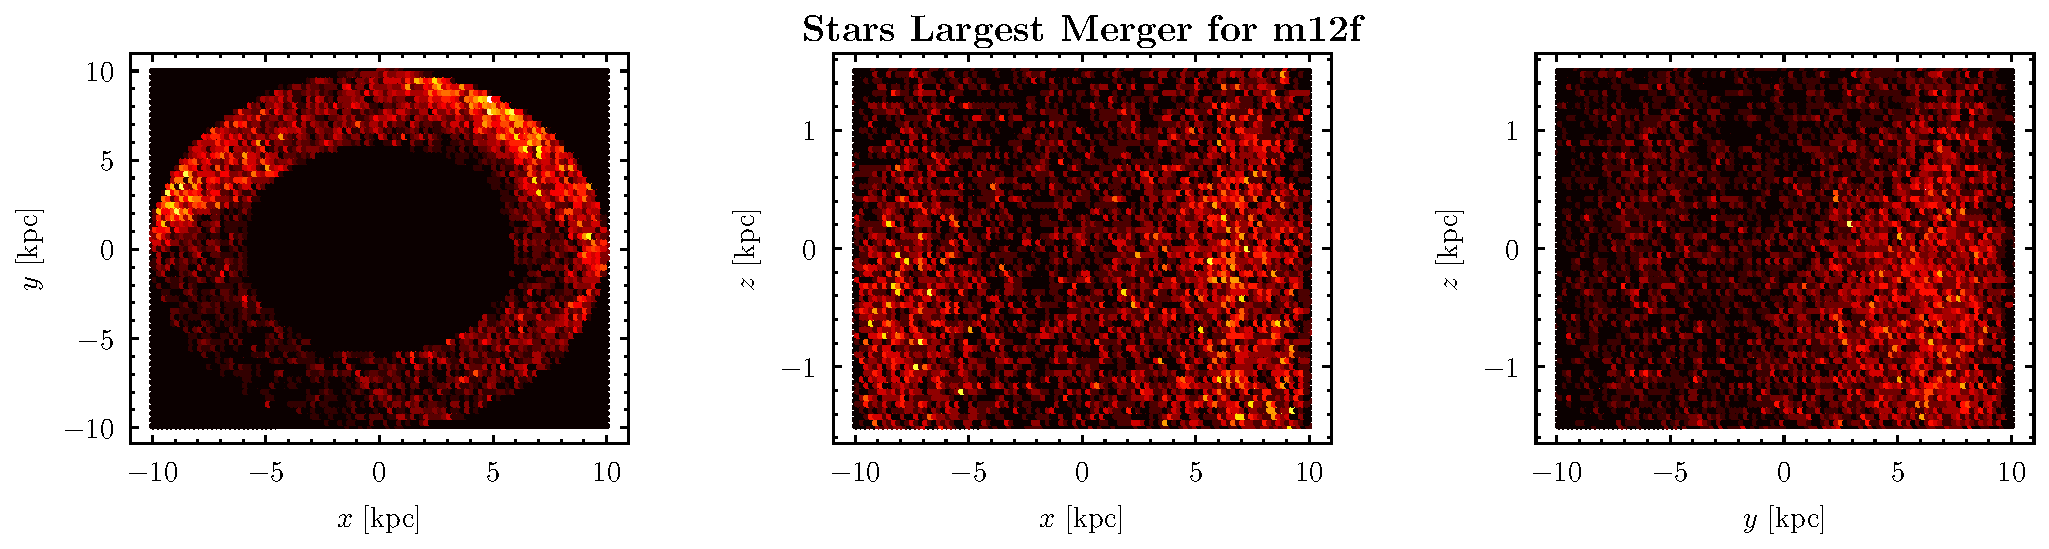
\includegraphics[width=6in]{plots/starsstar_dm_2d_pos_merger_0m12f.pdf} 
% 	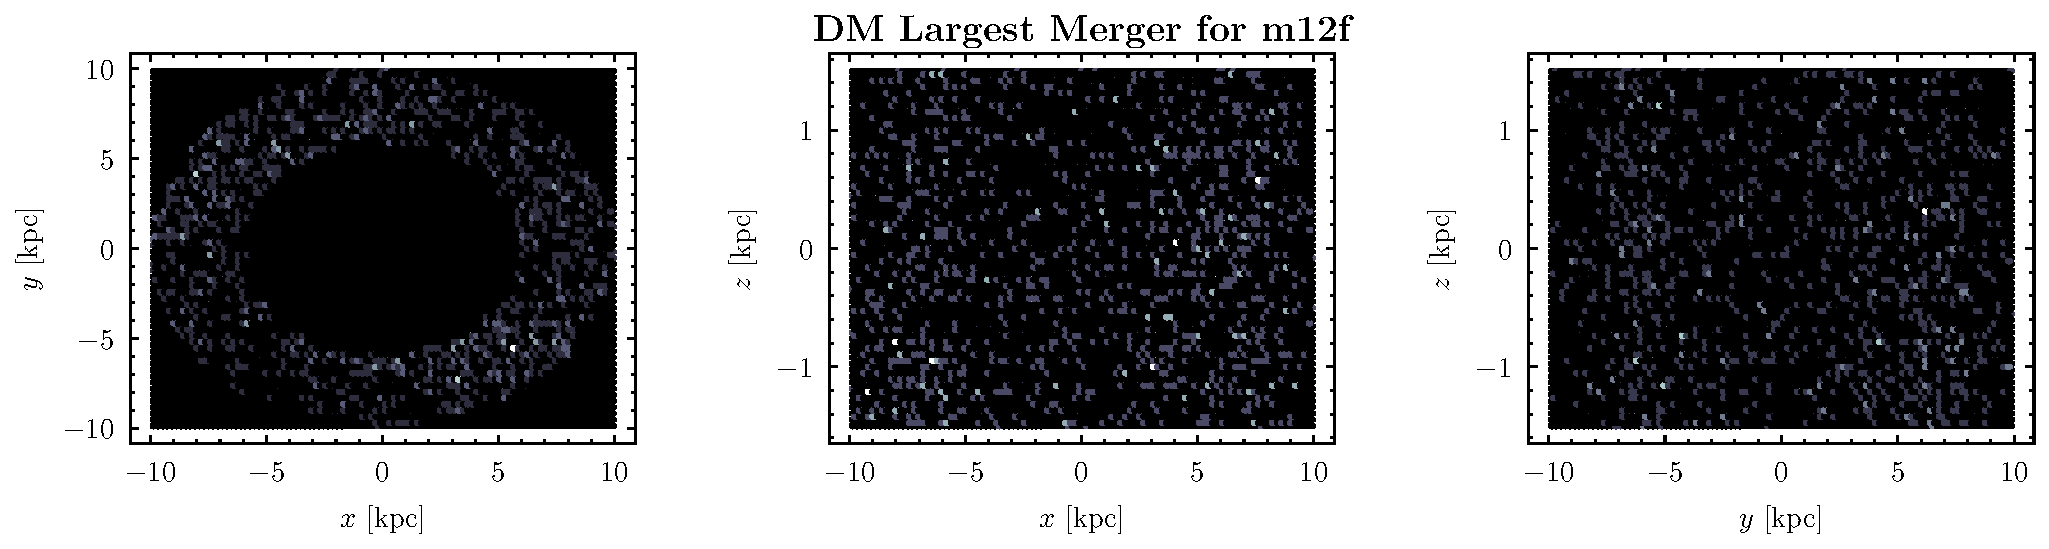
\includegraphics[width=6in]{plots/darkstar_dm_2d_pos_merger_0m12f.pdf} 
%   \caption{Position distributions for the largest merger of simulations \texttt{m12f} for stars (top) and DM (bottom).}
%   \label{fig:m12f_position}
%\end{figure*}




\begin{figure*}[h] %  figure placement: here, top, bottom, or page
   \centering
	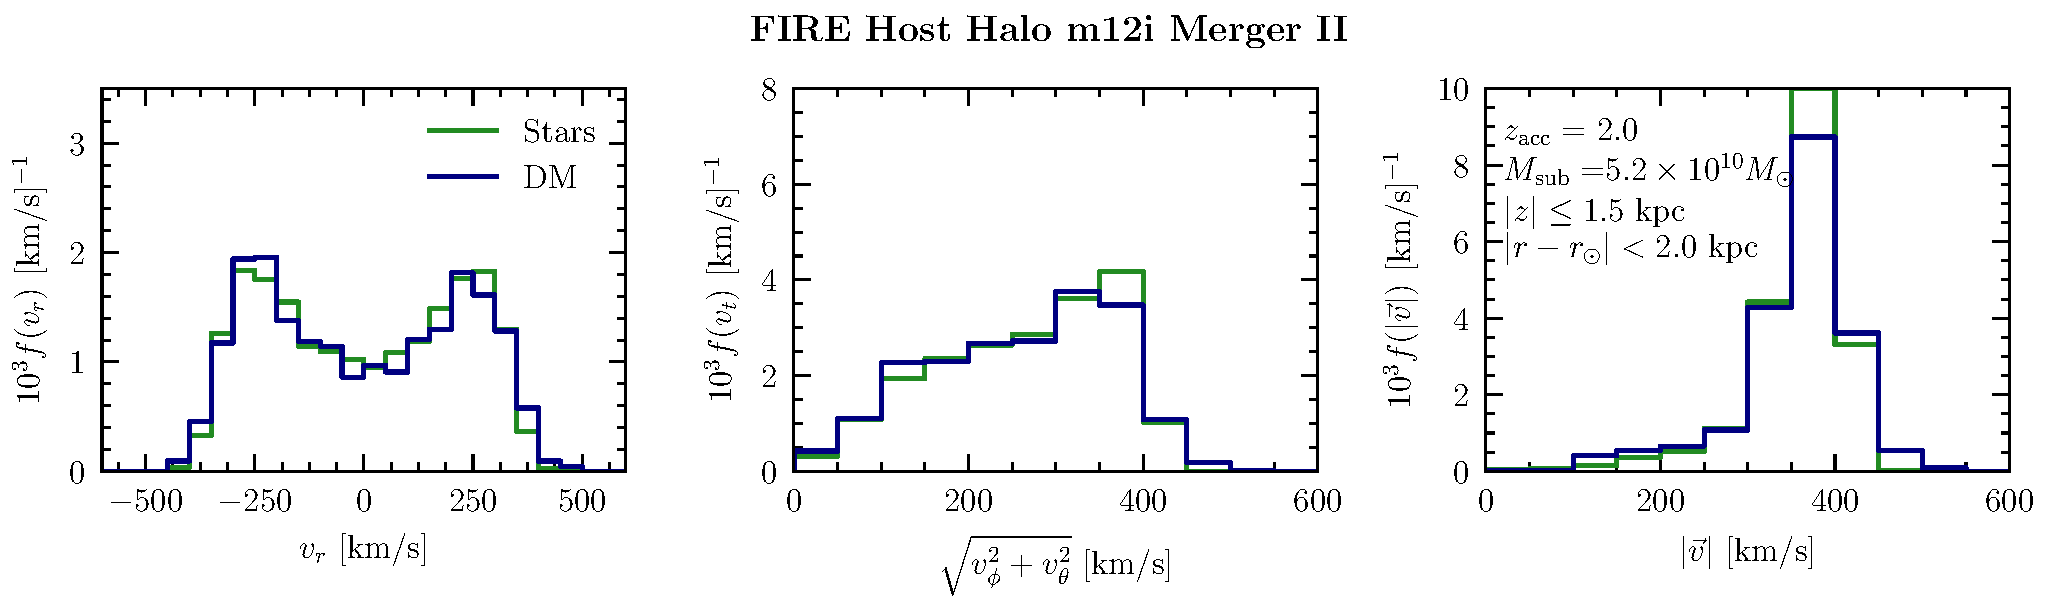
\includegraphics[width=7in]{plots/star_dm_vr_vt_v_merger_1m12i.pdf} 
	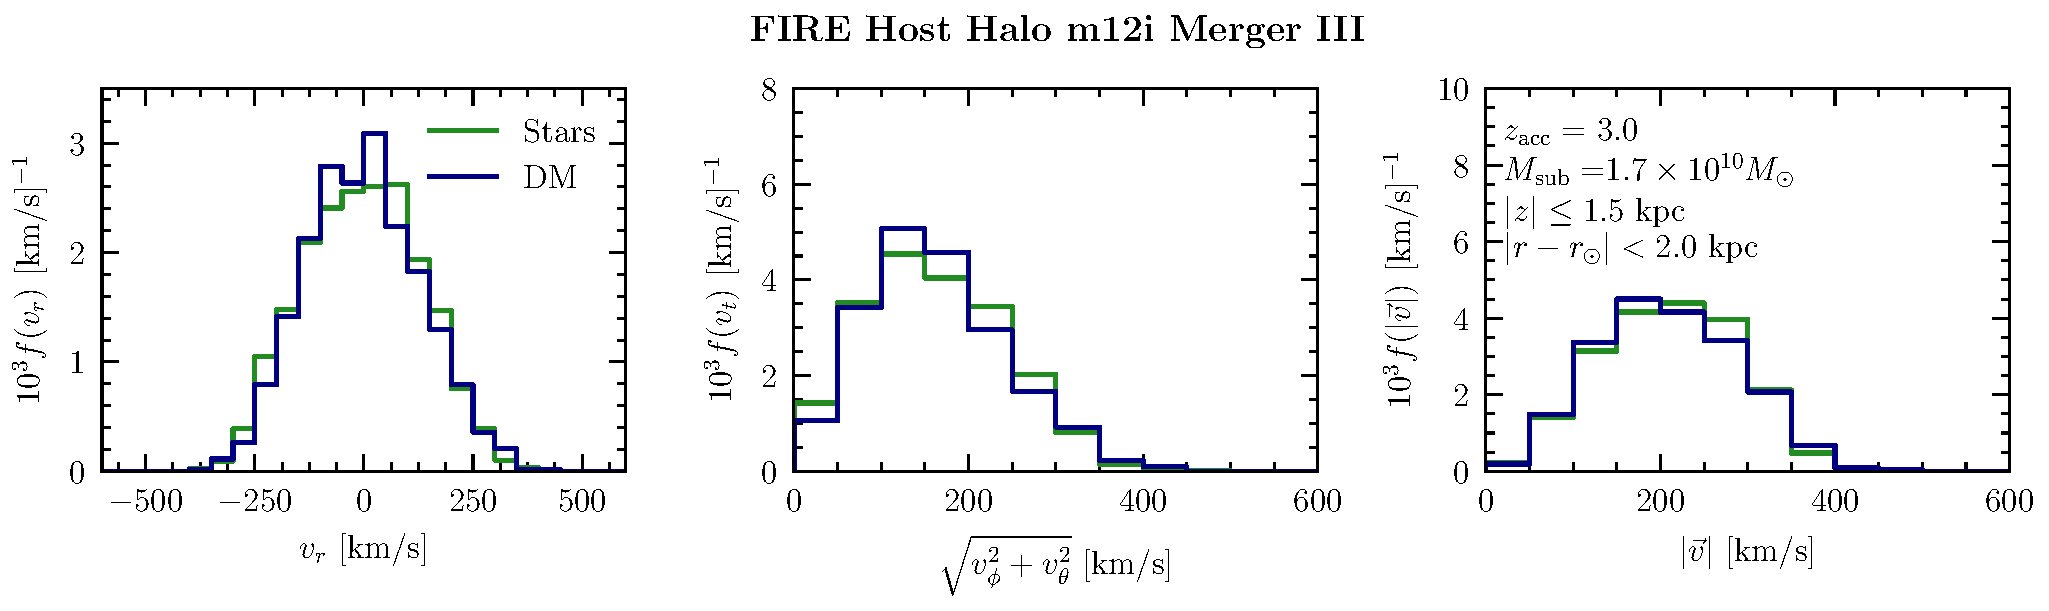
\includegraphics[width=7in]{plots/star_dm_vr_vt_v_merger_2m12i.pdf} 
	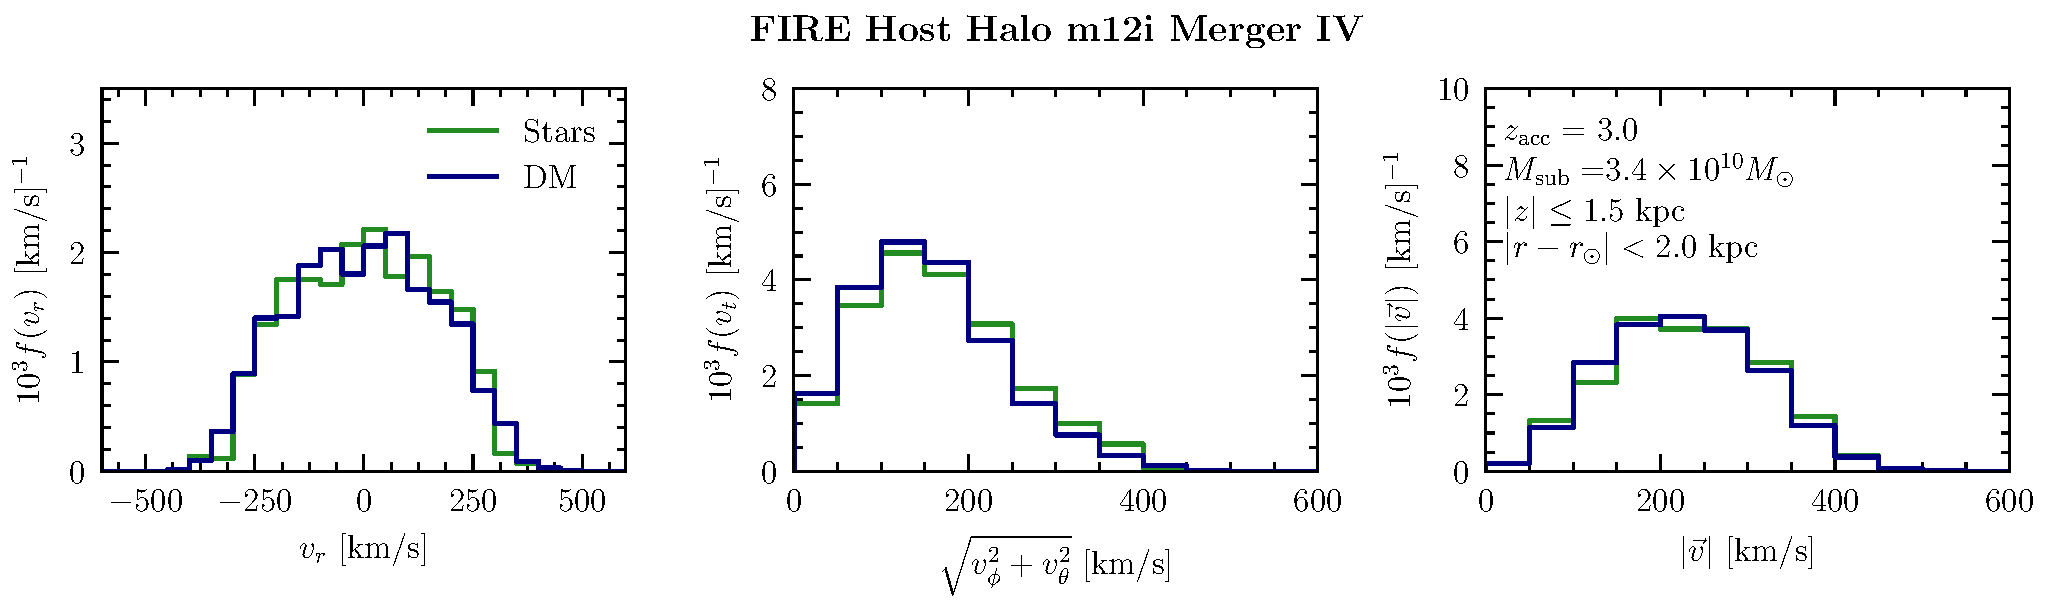
\includegraphics[width=7in]{plots/star_dm_vr_vt_v_merger_3m12i.pdf} 
   \caption{Velocity component distributions for the second, third, and fourth largest merger of simulations \texttt{m12i} by stellar mass. }
   \label{fig:other_mergers}
\end{figure*}


\begin{figure*}[h] %  figure placement: here, top, bottom, or page
   \centering
	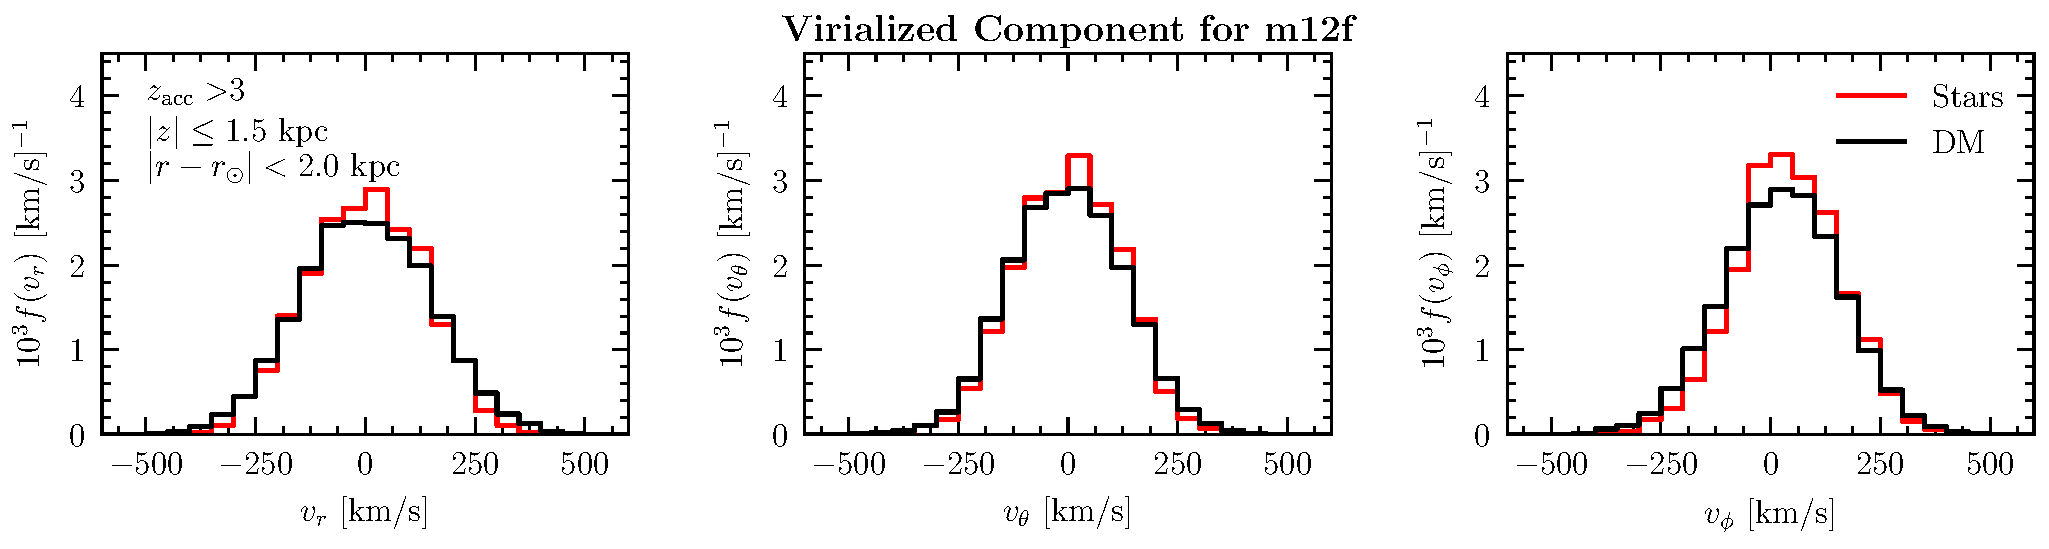
\includegraphics[width=7in]{plots/virialized_component_vr_vtheta_vphi3m12f.pdf} 
   \caption{Velocity distributions of all accreted particles in \mf~that merged at $z_{\rm{acc}} > 3$, similar to \Fig{fig:virialized}.}
   \label{fig:virialized_m12f}
\end{figure*}


%\begin{figure*}[tb] %  figure placement: here, top, bottom, or page
%   \centering
%		\includegraphics[width=6in]{plots/{component_star_dmz_cut1.5d_cut2.0radialredshift0.88m12f}.pdf} 
%		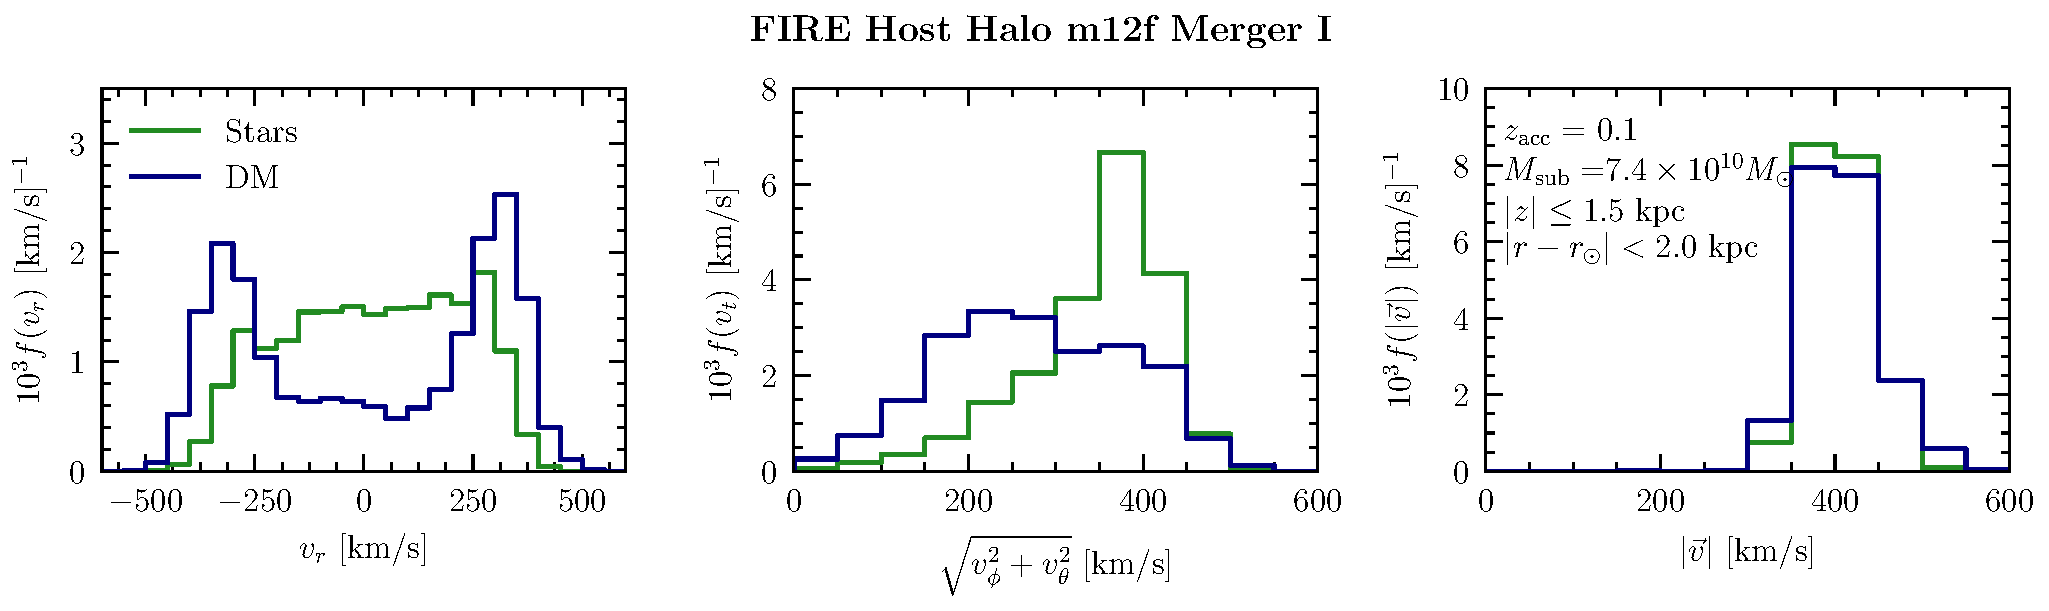
\includegraphics[width=6in]{plots/star_dm_vr_vt_v_merger_0m12f.pdf} 
%		\includegraphics[width=6in]{plots/{component_star_dm_no_mergerz_cut1.5d_cut2.0radialredshift0.09m12f}.pdf} 
%   \caption{Velocity component distribution for m12f}
%   \label{fig:velocity_components_m12f}
%\end{figure*}



\end{document} 





